% Generated by Sphinx.
\def\sphinxdocclass{report}
\documentclass[letterpaper,10pt,english]{sphinxmanual}
\usepackage[utf8]{inputenc}
\DeclareUnicodeCharacter{00A0}{\nobreakspace}
\usepackage[T1]{fontenc}
\usepackage{babel}
\usepackage{times}
\usepackage[Bjarne]{fncychap}
\usepackage{longtable}
\usepackage{sphinx}


\title{Cuckoo Sandbox Book}
\date{December 26, 2011}
\release{0.3}
\author{Cuckoo Sandbox}
\newcommand{\sphinxlogo}{}
\renewcommand{\releasename}{Release}
\makeindex

\makeatletter
\def\PYG@reset{\let\PYG@it=\relax \let\PYG@bf=\relax%
    \let\PYG@ul=\relax \let\PYG@tc=\relax%
    \let\PYG@bc=\relax \let\PYG@ff=\relax}
\def\PYG@tok#1{\csname PYG@tok@#1\endcsname}
\def\PYG@toks#1+{\ifx\relax#1\empty\else%
    \PYG@tok{#1}\expandafter\PYG@toks\fi}
\def\PYG@do#1{\PYG@bc{\PYG@tc{\PYG@ul{%
    \PYG@it{\PYG@bf{\PYG@ff{#1}}}}}}}
\def\PYG#1#2{\PYG@reset\PYG@toks#1+\relax+\PYG@do{#2}}

\def\PYG@tok@gd{\def\PYG@tc##1{\textcolor[rgb]{0.63,0.00,0.00}{##1}}}
\def\PYG@tok@gu{\let\PYG@bf=\textbf\def\PYG@tc##1{\textcolor[rgb]{0.50,0.00,0.50}{##1}}}
\def\PYG@tok@gt{\def\PYG@tc##1{\textcolor[rgb]{0.00,0.25,0.82}{##1}}}
\def\PYG@tok@gs{\let\PYG@bf=\textbf}
\def\PYG@tok@gr{\def\PYG@tc##1{\textcolor[rgb]{1.00,0.00,0.00}{##1}}}
\def\PYG@tok@cm{\let\PYG@it=\textit\def\PYG@tc##1{\textcolor[rgb]{0.25,0.50,0.56}{##1}}}
\def\PYG@tok@vg{\def\PYG@tc##1{\textcolor[rgb]{0.73,0.38,0.84}{##1}}}
\def\PYG@tok@m{\def\PYG@tc##1{\textcolor[rgb]{0.13,0.50,0.31}{##1}}}
\def\PYG@tok@mh{\def\PYG@tc##1{\textcolor[rgb]{0.13,0.50,0.31}{##1}}}
\def\PYG@tok@cs{\def\PYG@tc##1{\textcolor[rgb]{0.25,0.50,0.56}{##1}}\def\PYG@bc##1{\colorbox[rgb]{1.00,0.94,0.94}{##1}}}
\def\PYG@tok@ge{\let\PYG@it=\textit}
\def\PYG@tok@vc{\def\PYG@tc##1{\textcolor[rgb]{0.73,0.38,0.84}{##1}}}
\def\PYG@tok@il{\def\PYG@tc##1{\textcolor[rgb]{0.13,0.50,0.31}{##1}}}
\def\PYG@tok@go{\def\PYG@tc##1{\textcolor[rgb]{0.19,0.19,0.19}{##1}}}
\def\PYG@tok@cp{\def\PYG@tc##1{\textcolor[rgb]{0.00,0.44,0.13}{##1}}}
\def\PYG@tok@gi{\def\PYG@tc##1{\textcolor[rgb]{0.00,0.63,0.00}{##1}}}
\def\PYG@tok@gh{\let\PYG@bf=\textbf\def\PYG@tc##1{\textcolor[rgb]{0.00,0.00,0.50}{##1}}}
\def\PYG@tok@ni{\let\PYG@bf=\textbf\def\PYG@tc##1{\textcolor[rgb]{0.84,0.33,0.22}{##1}}}
\def\PYG@tok@nl{\let\PYG@bf=\textbf\def\PYG@tc##1{\textcolor[rgb]{0.00,0.13,0.44}{##1}}}
\def\PYG@tok@nn{\let\PYG@bf=\textbf\def\PYG@tc##1{\textcolor[rgb]{0.05,0.52,0.71}{##1}}}
\def\PYG@tok@no{\def\PYG@tc##1{\textcolor[rgb]{0.38,0.68,0.84}{##1}}}
\def\PYG@tok@na{\def\PYG@tc##1{\textcolor[rgb]{0.25,0.44,0.63}{##1}}}
\def\PYG@tok@nb{\def\PYG@tc##1{\textcolor[rgb]{0.00,0.44,0.13}{##1}}}
\def\PYG@tok@nc{\let\PYG@bf=\textbf\def\PYG@tc##1{\textcolor[rgb]{0.05,0.52,0.71}{##1}}}
\def\PYG@tok@nd{\let\PYG@bf=\textbf\def\PYG@tc##1{\textcolor[rgb]{0.33,0.33,0.33}{##1}}}
\def\PYG@tok@ne{\def\PYG@tc##1{\textcolor[rgb]{0.00,0.44,0.13}{##1}}}
\def\PYG@tok@nf{\def\PYG@tc##1{\textcolor[rgb]{0.02,0.16,0.49}{##1}}}
\def\PYG@tok@si{\let\PYG@it=\textit\def\PYG@tc##1{\textcolor[rgb]{0.44,0.63,0.82}{##1}}}
\def\PYG@tok@s2{\def\PYG@tc##1{\textcolor[rgb]{0.25,0.44,0.63}{##1}}}
\def\PYG@tok@vi{\def\PYG@tc##1{\textcolor[rgb]{0.73,0.38,0.84}{##1}}}
\def\PYG@tok@nt{\let\PYG@bf=\textbf\def\PYG@tc##1{\textcolor[rgb]{0.02,0.16,0.45}{##1}}}
\def\PYG@tok@nv{\def\PYG@tc##1{\textcolor[rgb]{0.73,0.38,0.84}{##1}}}
\def\PYG@tok@s1{\def\PYG@tc##1{\textcolor[rgb]{0.25,0.44,0.63}{##1}}}
\def\PYG@tok@gp{\let\PYG@bf=\textbf\def\PYG@tc##1{\textcolor[rgb]{0.78,0.36,0.04}{##1}}}
\def\PYG@tok@sh{\def\PYG@tc##1{\textcolor[rgb]{0.25,0.44,0.63}{##1}}}
\def\PYG@tok@ow{\let\PYG@bf=\textbf\def\PYG@tc##1{\textcolor[rgb]{0.00,0.44,0.13}{##1}}}
\def\PYG@tok@sx{\def\PYG@tc##1{\textcolor[rgb]{0.78,0.36,0.04}{##1}}}
\def\PYG@tok@bp{\def\PYG@tc##1{\textcolor[rgb]{0.00,0.44,0.13}{##1}}}
\def\PYG@tok@c1{\let\PYG@it=\textit\def\PYG@tc##1{\textcolor[rgb]{0.25,0.50,0.56}{##1}}}
\def\PYG@tok@kc{\let\PYG@bf=\textbf\def\PYG@tc##1{\textcolor[rgb]{0.00,0.44,0.13}{##1}}}
\def\PYG@tok@c{\let\PYG@it=\textit\def\PYG@tc##1{\textcolor[rgb]{0.25,0.50,0.56}{##1}}}
\def\PYG@tok@mf{\def\PYG@tc##1{\textcolor[rgb]{0.13,0.50,0.31}{##1}}}
\def\PYG@tok@err{\def\PYG@bc##1{\fcolorbox[rgb]{1.00,0.00,0.00}{1,1,1}{##1}}}
\def\PYG@tok@kd{\let\PYG@bf=\textbf\def\PYG@tc##1{\textcolor[rgb]{0.00,0.44,0.13}{##1}}}
\def\PYG@tok@ss{\def\PYG@tc##1{\textcolor[rgb]{0.32,0.47,0.09}{##1}}}
\def\PYG@tok@sr{\def\PYG@tc##1{\textcolor[rgb]{0.14,0.33,0.53}{##1}}}
\def\PYG@tok@mo{\def\PYG@tc##1{\textcolor[rgb]{0.13,0.50,0.31}{##1}}}
\def\PYG@tok@mi{\def\PYG@tc##1{\textcolor[rgb]{0.13,0.50,0.31}{##1}}}
\def\PYG@tok@kn{\let\PYG@bf=\textbf\def\PYG@tc##1{\textcolor[rgb]{0.00,0.44,0.13}{##1}}}
\def\PYG@tok@o{\def\PYG@tc##1{\textcolor[rgb]{0.40,0.40,0.40}{##1}}}
\def\PYG@tok@kr{\let\PYG@bf=\textbf\def\PYG@tc##1{\textcolor[rgb]{0.00,0.44,0.13}{##1}}}
\def\PYG@tok@s{\def\PYG@tc##1{\textcolor[rgb]{0.25,0.44,0.63}{##1}}}
\def\PYG@tok@kp{\def\PYG@tc##1{\textcolor[rgb]{0.00,0.44,0.13}{##1}}}
\def\PYG@tok@w{\def\PYG@tc##1{\textcolor[rgb]{0.73,0.73,0.73}{##1}}}
\def\PYG@tok@kt{\def\PYG@tc##1{\textcolor[rgb]{0.56,0.13,0.00}{##1}}}
\def\PYG@tok@sc{\def\PYG@tc##1{\textcolor[rgb]{0.25,0.44,0.63}{##1}}}
\def\PYG@tok@sb{\def\PYG@tc##1{\textcolor[rgb]{0.25,0.44,0.63}{##1}}}
\def\PYG@tok@k{\let\PYG@bf=\textbf\def\PYG@tc##1{\textcolor[rgb]{0.00,0.44,0.13}{##1}}}
\def\PYG@tok@se{\let\PYG@bf=\textbf\def\PYG@tc##1{\textcolor[rgb]{0.25,0.44,0.63}{##1}}}
\def\PYG@tok@sd{\let\PYG@it=\textit\def\PYG@tc##1{\textcolor[rgb]{0.25,0.44,0.63}{##1}}}

\def\PYGZbs{\char`\\}
\def\PYGZus{\char`\_}
\def\PYGZob{\char`\{}
\def\PYGZcb{\char`\}}
\def\PYGZca{\char`\^}
\def\PYGZsh{\char`\#}
\def\PYGZpc{\char`\%}
\def\PYGZdl{\char`\$}
\def\PYGZti{\char`\~}
% for compatibility with earlier versions
\def\PYGZat{@}
\def\PYGZlb{[}
\def\PYGZrb{]}
\makeatother

\begin{document}

\maketitle
\tableofcontents
\phantomsection\label{index::doc}


Cuckoo Sandbox is an \emph{Open Source} software for automating analysis of suspicious files.
To do so it makes use of custom components that monitor the behavior of the malicious
processes while running in an isolated Windows environment.

This book explains what Cuckoo is, how it works and what you can do with it, from
setup and run Cuckoo to how to customize it and extend it.


\chapter{Having troubles?}
\label{index:index}\label{index:cuckoo-sandbox-book}\label{index:having-troubles}
If you're having troubles you might want to check out the {\hyperref[faq/index::doc]{\emph{FAQ}}}
it might already have the answers to your questions.


\section{FAQ}
\label{faq/index:faq}\label{faq/index::doc}
Frequently Asked Questions:
\begin{itemize}
\item {} 
{\hyperref[faq/index:question-1]{\emph{How to start an analysis?}}}

\item {} 
{\hyperref[faq/index:question-2]{\emph{How to change Cuckoo default behaviour?}}}

\item {} 
{\hyperref[faq/index:question-3]{\emph{Can I redistribute Cuckoo Sandbox?}}}

\item {} 
{\hyperref[faq/index:question-4]{\emph{Can I include Cuckoo Sandbox in my closed source commercial product?}}}

\item {} 
{\hyperref[faq/index:question-5]{\emph{I want to help Cuckoo, what can I do?}}}

\item {} 
{\hyperref[faq/index:question-6]{\emph{I want to help but I don't have time}}}

\end{itemize}


\subsection{Usage questions}
\label{faq/index:usage-questions}

\subsubsection{How to start an analysis?}
\label{faq/index:question-1}\label{faq/index:how-to-start-an-analysis}
You can simply start an analysis via command-line utility \code{submit.py}.
Check {\hyperref[usage/submit::doc]{\emph{Submit an analysis}}}.


\subsubsection{How to change Cuckoo default behaviour?}
\label{faq/index:how-to-change-cuckoo-default-behaviour}\label{faq/index:question-2}
Depending on what you mean, you can edit Cuckoo's configuration files (see
{\hyperref[installation/host/configuration::doc]{\emph{Configuration}}}) or work on the analysis packages
(see {\hyperref[customization/packages::doc]{\emph{Analysis Packages}}}).


\subsection{General questions}
\label{faq/index:general-questions}

\subsubsection{Can I redistribute Cuckoo Sandbox?}
\label{faq/index:question-3}\label{faq/index:can-i-redistribute-cuckoo-sandbox}
Yes, you can. Cuckoo Sandbox is distributed under the GNU General Public
License version 3. See {\hyperref[introduction/license::doc]{\emph{License}}}.


\subsubsection{Can I include Cuckoo Sandbox in my closed source commercial product?}
\label{faq/index:can-i-include-cuckoo-sandbox-in-my-closed-source-commercial-product}\label{faq/index:question-4}
Generally no, you can't. Cuckoo Sandbox is distributed under the GNU General
Public License version 3. See {\hyperref[introduction/license::doc]{\emph{License}}}.


\subsubsection{I want to help Cuckoo, what can I do?}
\label{faq/index:i-want-to-help-cuckoo-what-can-i-do}\label{faq/index:question-5}
Your help is very appreciated, you can help Cuckoo Sandbox in several ways,
from coding to send bug reports. See {\hyperref[finalremarks/index::doc]{\emph{Final Remarks}}}.


\subsubsection{I want to help but I don't have time}
\label{faq/index:i-want-to-help-but-i-don-t-have-time}\label{faq/index:question-6}
There are many ways to help Cuckoo: coding, testing, reporting bugs, donating
money or hardware, reviewing code and documentation or submitting feature
requests or feedback.
Just do whatever you feel could help the project with your possibilities.

Otherwise you can ask to the developers and to other Cuckoo users in the
\#cuckoobox IRC channel.


\chapter{Contents}
\label{index:cuckoobox}\label{index:contents}

\section{Introduction}
\label{introduction/index:introduction}\label{introduction/index::doc}
This is an introductory chapter to Cuckoo Sandbox.
It explains some basic malware analysis concepts, what's Cuckoo an how it can fit in malware analysis.


\subsection{Sandboxing}
\label{introduction/sandboxing:sandboxing}\label{introduction/sandboxing::doc}
As defined by \href{http://en.wikipedia.org/wiki/Sandbox\_\%28computer\_security\%29}{Wikipedia}, ``\emph{in computer security, a sandbox is a security
mechanism for separating running programs. It is often used to execute untested
code, or untrusted programs from unverified third-parties, suppliers, untrusted
users and untrusted websites.}''.

This concept applies to malware analysis' sandboxing too: our goal is to run an
unknown and untrusted application or file inside an isolated environment and get
information and what it does.

Malware sandboxing is a practical application of the dynamical analysis
approach: instead of statically analyze the binary file, it gets executed and
monitored in real-time.

This approach obviously has pros and cons, but it's a valuable technique to
obtain additional details on the malware, such as its network behavior.
Therefore it's a good practice to perform both static and dynamic analysis while
inspecting a malware, in order to gain a deeper understanding of it.

Simple as it is, Cuckoo is a tool that allows you to perform sandboxed malware
analysis.


\subsubsection{Using a Sandbox}
\label{introduction/sandboxing:wikipedia}\label{introduction/sandboxing:using-a-sandbox}
Before starting installing, configuring and using Cuckoo you should take some
time to think on what you want to achieve with it and how.

Some questions you should ask yourself:
\begin{itemize}
\item {} 
What kind of files do I want to analyze?

\item {} 
Which volumes of analysis do I want to be able to handle?

\item {} 
Which platform do I want to use to run my analysis on?

\item {} 
What kind of information I want about the file?

\end{itemize}

The creation of the isolated environment (the virtual machine) is probably the
most critical and important part of a sandbox deployment: it should be done
carefully and with proper planning.

Before getting hands on the virtualization product of your choice, you should
already have a design plan that defines:
\begin{itemize}
\item {} 
Which operating system, language and patching level to use.

\item {} 
Which softwares to install and which versions (particularly important when analyzing exploits).

\end{itemize}

Consider that automated malware analysis is not deterministic and its success
might depend on a trillion of factors: you are trying to make a malware run
in a virtualized system as it would do on a native one, which could be tricky to
achieve and could not always succeed.
Your goal should be both to create a system able to handle all the requirements
you need as well as try to make it as realistic as possible.

For example you could consider leaving some intentional traces of normal usage,
such as browsing history, cookies, documents, images etc. If a malware is
designed to operate, manipulate or steal such files you'll be able to notice it.

Virtualized operating systems usually carry a lot of traces with them that makes
them very easily detectable. Even if you shouldn't overestimate this problem,
you might want to take care of this and try to hide as many virtualization
traces as possible.
There is a lot of literature on Internet regarding virtualization detection
techniques and countermeasures.

Once you finished designing and preparing the prototype of system you want, you
can proceed creating it and deploying it. You will be always in time to
change things or slightly fix them, but remember that good planning at the
beginning always means less troubles in the long run.


\subsection{What is Cuckoo?}
\label{introduction/what::doc}\label{introduction/what:what-is-cuckoo}
Cuckoo is an open source automated malware analysis system.

It's used to automatically run and analyze files and collect comprehensive
analysis results that outline what the malware does while running inside an
isolated Windows operating system.

It can retrieve the following type of results:
\begin{itemize}
\item {} 
Traces of win32 API calls performed by all processes spawned by the malware.

\item {} 
Files being created, deleted and downloaded by the malware during its execution.

\item {} 
Network traffic trace in PCAP format.

\item {} 
Screenshots of Windows desktop taken during the execution of the malware.

\item {} 
Traces of assembly instructions performed by the malware.

\end{itemize}


\subsubsection{Some History}
\label{introduction/what:some-history}
Cuckoo Sandbox started as a \href{http://www.google-melange.com}{Google Summer of Code} project in 2010 within
\href{http://www.honeynet.org}{The Honeynet Project}.
It was originally designed and developed by \emph{Claudio “nex” Guarnieri}, who still
mantains it and coordinates all efforts from joined developers and contributors.

After initial work during the summer 2010, the first beta release was published
on Feb. 5th 2011, when Cuckoo was publicly announced and distributed for the
first time.

In March 2011, Cuckoo as been selected again as a supported project during
Google Summer of Code 2011 with The Honeynet Project, during which
\emph{Dario Fernandes} joined the project and extended its functionalities.

On November 2nd 2011 Cuckoo the release of its 0.2 version to the public as the
first real stable release.

On late November 2011 \emph{Alessandro ``jekil'' Tanasi} joined the team expanding
Cuckoo's processing and reporting functionalities.

On December 2011 Cuckoo v0.3 gets released.


\subsubsection{Use Cases}
\label{introduction/what:the-honeynet-project}\label{introduction/what:use-cases}
Cuckoo is designed to be used both as a standalone application as well as to be
integrated in larger frameworks, thanks to its submission and processing
automation capabilities.

It can be used to analyze:
\begin{itemize}
\item {} 
Generic Windows executables

\item {} 
DLL files

\item {} 
PDF documents

\item {} 
Microsoft Office documents

\item {} 
URLs

\item {} 
PHP scripts

\item {} 
\emph{Almost everything else}

\end{itemize}

Thanks to its scripting and customization capabilities there's basically no
limit to what you can achieve with Cuckoo, for example automating malware
unpacking or automating the dump of configuration files and web-injects
from banking trojans.

For more information on customizing Cuckoo, see the {\hyperref[customization/index::doc]{\emph{Customization}}}
chapter.


\subsubsection{Architecture}
\label{introduction/what:architecture}
Cuckoo Sandbox consists of a central management software which handles sample
execution and analysis.

Each analysis is launched in a fresh and isolated virtual machine.
Cuckoo's infrastructure is composed by an Host machine (the management
software) and a number of Guest machines (virtual machines for analysis).

The Host runs the core component of the sandbox that manages the whole
analysis and execution process, while the Guests are the isolated environments
where the malwares get actually safely executed and analyzed.

The following picture explains Cuckoo's architecture:
\begin{quote}
\begin{figure}[htbp]
\centering

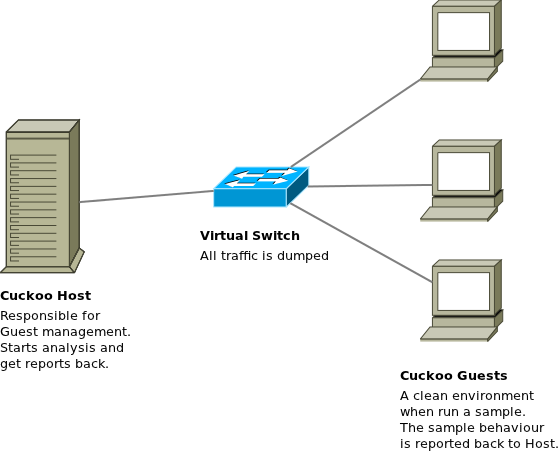
\includegraphics{architecture.png}
\end{figure}
\end{quote}

Although recommended setup is \emph{GNU/Linux} (Ubuntu preferrably) as host and
\emph{Windows XP Service Pack 3} as guest, Cuckoo proved to work smoothly also on
\emph{Mac OS X} as host and \emph{Windows Vista} and \emph{Windows 7} as guests.


\subsubsection{Obtaining Cuckoo}
\label{introduction/what:obtaining-cuckoo}
Cuckoo can be downloaded from the \href{http://www.cuckoobox.org}{official website}, where the stable and
packaged releases are distributed, or can be cloned from our \href{http://github.com/cuckoobox/cuckoo}{official git
repository}.
\begin{quote}

\begin{notice}{warning}{Warning:}
While being more updated, including new features and bugfixes, the
version available in the git repository should be considered an
\emph{under development} stage. Therefore its stability is not guaranteed
and it most likely lacks updated documentation.
\end{notice}
\end{quote}


\subsection{License}
\label{introduction/license:official-git-repository}\label{introduction/license::doc}\label{introduction/license:license}
Cuckoo Sandbox is copyrighted by \emph{Claudio Guarnieri} and is licensed under GNU
General Public License version 3.

Cuckoo Sandbox is free software: you can redistribute it and/or modify
it under the terms of GNU General Public License as published by the Free
Software Foundation, either version 3 of the License, or (at your opinion) any
later version.

See the \href{http://www.gnu.org/licenses/gpl.txt}{GNU General Public License} for more details.


\subsection{Disclaimer}
\label{introduction/license:gnu-general-public-license}\label{introduction/license:disclaimer}
Cuckoo is distributed as it is, in the hope that it will be useful, but without
any warranty neither the implied merchantability or fitness for a particular
purpose.

Whatever you do with this tool is uniquely your own responsibility.


\section{Installation}
\label{installation/index:installation}\label{installation/index::doc}
This chapter explains how to install Cuckoo.

\begin{notice}{note}{Note:}
This documentation refers to \emph{Host} as the underlying operating systems on
which you are running Cuckoo (generally being a GNU/Linux distribution) and
to \emph{Guest} as the Windows virtual machine used to run the isolated analysis.
\end{notice}


\subsection{Preparing the Host}
\label{installation/host/index:preparing-the-host}\label{installation/host/index::doc}
Even though it's reported to run on other operating systems too, Cuckoo is
originally supposed to run on a \emph{GNU/Linux} native system.
For the purpose of this documentation, we chose \textbf{latest Ubuntu LTS} as
reference system for the commands examples.


\subsubsection{Requirements}
\label{installation/host/requirements:requirements}\label{installation/host/requirements::doc}
Before proceeding on configuring Cuckoo, you'll need to install some required
software and libraries.


\paragraph{Installing Python libraries}
\label{installation/host/requirements:installing-python-libraries}
Cuckoo host components are completely written in Python, therefore make sure to
have an appropriate version installed. For current release Python 2.6 or 2.7 are
preferred.

Install Python on Ubuntu:

\begin{Verbatim}[commandchars=@\[\]]
@$ sudo apt-get install python
\end{Verbatim}

Cuckoo makes use of several libraries which include:
\begin{itemize}
\item {} 
\href{http://www.darwinsys.com/file/}{Magic}: for detecting file types.

\item {} 
\href{http://code.google.com/p/dpkt/}{Dpkt}: for extracting relevant information from PCAP files.

\item {} 
\href{http://www.makotemplates.org}{Mako}: for rendering the HTML reports and the web interface.

\end{itemize}

On Ubuntu you can install all of them with the following command:

\begin{Verbatim}[commandchars=@\[\]]
@$ sudo apt-get install python-magic python-dpkt python-mako
\end{Verbatim}

On different distributions refer to the provided official homepage to retrieve
other installers or sources.

Other optional libraries, which do not affect Cuckoo's execution, include:
\begin{itemize}
\item {} 
\href{http://code.google.com/p/pyssdeep/}{Pyssdeep}: for calculating ssdeep fuzzy hash of files.

\end{itemize}


\paragraph{Installing VirtualBox}
\label{installation/host/requirements:pyssdeep}\label{installation/host/requirements:installing-virtualbox}
At current stage, Cuckoo heavily relies on \href{http://www.virtualbox.org}{VirtualBox} as it's unique
virtualization engine.

Despite being often packaged by all GNU/Linux distributions, you are encouraged
to download and install the latest version from the official website. The reason
behind this choice is that packaged versions of VirtualBox (called OSE)
generally have some limitations or adjustments in order to meet requirements of
the GNU GPL license.

You can get the proper package for your distribution at the \href{https://www.virtualbox.org/wiki/Linux\_Downloads}{official download
page}.

The installation of VirtualBox is not in purposes of this documentation, if you
are not familiar with it please refer to the \href{https://www.virtualbox.org/wiki/Documentation}{official documentation}.


\paragraph{Installing Tcpdump}
\label{installation/host/requirements:installing-tcpdump}\label{installation/host/requirements:official-documentation}
By default Cuckoo makes use of VirtualBox's embedded network tracing
functionalities, but in some cases or some network configurations you might need
to adopt an external network sniffer.

If you intend to use VirtualBox's own network trace, you can skip this section.

The best choice for packet interception is \href{http://www.tcpdump.org}{tcpdump} of course.

Install it on Ubuntu:

\begin{Verbatim}[commandchars=@\[\]]
@$ sudo apt-get install tcpdump
\end{Verbatim}

Tcpdump requires root privileges, but since you don't want Cuckoo to run as root
you'll have to set specific Linux capabilities to the binary:

\begin{Verbatim}[commandchars=@\[\]]
@$ sudo setcap cap@_net@_raw,cap@_net@_admin=eip /usr/sbin/tcpdump
\end{Verbatim}

You can verify the results of last command with:

\begin{Verbatim}[commandchars=@\[\]]
@$ getcap /usr/sbin/tcpdump
/usr/sbin/tcpdump = cap@_net@_admin,cap@_net@_raw+eip
\end{Verbatim}


\subsubsection{Installing Cuckoo}
\label{installation/host/installation::doc}\label{installation/host/installation:tcpdump}\label{installation/host/installation:installing-cuckoo}
Proceed with download and installation.


\paragraph{Create a user}
\label{installation/host/installation:create-a-user}
Even if you obviously can run Cuckoo with your current user, creating a dedicated
one is always a good practice.

Create a new user:

\begin{Verbatim}[commandchars=@\[\]]
@$ sudo adduser cuckoo
\end{Verbatim}

Make sure the new user belongs to the ``vboxusers'' group (or the group you used to
run VirtualBox):

\begin{Verbatim}[commandchars=@\[\]]
@$ sudo useradd -G vboxusers cuckoo
\end{Verbatim}


\paragraph{Download Cuckoo}
\label{installation/host/installation:download-cuckoo}
You can get your copy of Cuckoo from the \href{http://www.cuckoobox.org}{official website} or from our
\href{https://github.com/cuckoobox/cuckoo}{git repository}.

Please notice that the archives to be downloaded from the website are core
releases, while the version on git has to be considered an \textbf{under
development} stage, therefore possibly unstable and not yet fully documented.


\paragraph{Install it}
\label{installation/host/installation:install-it}\label{installation/host/installation:git-repository}
Extract or checkout your copy of Cuckoo to a path of your choice and you're
ready to go ;-).


\subsubsection{Configuration}
\label{installation/host/configuration:configuration}\label{installation/host/configuration::doc}
Cuckoo relies on two main configuration files:
\begin{itemize}
\item {} 
{\hyperref[installation/host/configuration:cuckoo-conf]{\emph{cuckoo.conf}}}: for configuring general behavior and analysis options.

\item {} 
{\hyperref[installation/host/configuration:reporting-conf]{\emph{reporting.conf}}}: for enabling or disabling report formats.

\end{itemize}


\paragraph{cuckoo.conf}
\label{installation/host/configuration:cuckoo-conf}\label{installation/host/configuration:id1}
We'll first start editing \emph{conf/cuckoo.conf} walking through every section and
option available.


\subparagraph{Logging}
\label{installation/host/configuration:logging}
Following is the logging section:

\begin{Verbatim}[commandchars=\\\{\}]
\PYG{p}{[}\PYG{n}{Logging}\PYG{p}{]}
\PYG{c}{\PYGZsh{} Enable/Disable additional debugging messages. This messages won't wrote to}
\PYG{c}{\PYGZsh{} log file but just printed on screen. [on/off]}
\PYG{n}{debug} \PYG{o}{=} \PYG{n}{off}
\end{Verbatim}

The \textbf{debug} option enables or disables debug messages that will be both printed
on standard output as well as stored in the log file.


\subparagraph{Analysis}
\label{installation/host/configuration:analysis}
Following is the analysis section:

\begin{Verbatim}[commandchars=@\[\]]
@PYGZlb[]Analysis@PYGZrb[]
@# This is the actual analysis timeout (expressed in seconds). This represents
@# the default timeout performed by analysis core if none is specified.
analysis@_timeout = 200
@# Watchdog timeout (expressed in seconds) for analysis execution to complete,
@# when this timeout gets hit, current execution is aborted and virtual machine
@# is restored and freed.
watchdog@_timeout = 600
@# Specify here the path where analysis results shall be stored.
results@_path = analysis/
\end{Verbatim}

This section defines two analysis time boundaries:
\begin{itemize}
\item {} 
\textbf{analysis timeout}: this timeout represent the maximum time an analysis should last, it can be overridden when submitting a file to analyze.

\item {} 
\textbf{watchdog timeout}: this is the time limit for which Cuckoo host should wait for the guest component (\emph{analyzer}) to terminate its operations.

\end{itemize}

The \emph{analysis timeout} should be smaller than the \emph{watchdog timeout}. If by
mistake it's configured differently, Cuckoo will force the \emph{analysis timeout}
to a smaller value.

Consider that the \emph{watchdog timeout} should be raised just under critical
circumstances, where the analyzer or virtual machine are not responding and
therefore need to be killed. When this happens, you'll most likely lose any
analysis results from that run.

The \textbf{results\_path} option defines where to store the analysis results.


\subparagraph{Processing}
\label{installation/host/configuration:processing}
Following is the processing section:

\begin{Verbatim}[commandchars=@\[\]]
@PYGZlb[]Processing@PYGZrb[]
@# Specify here the interpreter path to be used to launch the script.
interpreter = /usr/bin/python
@# Specify here the path to the analysis results processing script.
processor = processor.py
\end{Verbatim}

This section defines where the post-analysis processing script is located and
how it should be executed.

This script should be your interface to the analysis results and you should
use it and customize it at your will in order to consume the data generated by
Cuckoo. We'll get more into details on this in the {\hyperref[customization/index::doc]{\emph{Customization}}}
chapter.

By default Cuckoo provides a Python processing script that invokes some Python
classes used to process the results and to generate human readable analysis
reports (text, HTML, JSON).

The \textbf{interpreter} option defines the path to the application to be used to
execute the script.

The \textbf{processor} option defines the path to the script to be executed.


\subparagraph{Sniffer}
\label{installation/host/configuration:sniffer}
Following is the sniffer section:

\begin{Verbatim}[commandchars=@\[\]]
@PYGZlb[]Sniffer@PYGZrb[]
@# Enable or disable the following option by assigning a True or False value.
@# In case you decide to disable it, you're supposed to either not have any
@# network dump or to used VirtualBox's (or any other virtualization engine
@# you are using) to handle the network monitoring instead of using an external
@# sniffer such as tcpdump. @PYGZlb[]on/off@PYGZrb[]
sniffer = off
@# Path to the sniffer (tcpdump) binary.
path = /usr/sbin/tcpdump
@# This specifies the network interface where the sniffer will bind to in order
@# to monitor virtual machines' generated traffic.
interface = eth0
\end{Verbatim}

This section should be considered and edited just in the case you decided to use
an external sniffer (assuming that you {\hyperref[installation/host/requirements::doc]{\emph{properly installed}}}
it already).

If otherwise you don't plan to use an external sniffer, you can skip this section.

First you'll need to enable the \textbf{snifer} option by setting it to ``\emph{on}''.

The \textbf{path} option defines where the sniffer (tcpdump) binary is located. It
should be generally correct by default.

The \textbf{interface} option defines which network interface the sniffer should
monitor. This obviously depends on your network configuration and on how you
are planning to configure your virtual machines' networking. It's up to you.


\subparagraph{Virtual Machines}
\label{installation/host/configuration:virtual-machines}
Following is the Virtual Machines section:

\begin{Verbatim}[commandchars=@\[\]]
@PYGZlb[]VirtualMachines@PYGZrb[]
@# Virtualization product.
engine = VirtualBox
@# List virtual machines IDs separated by commas.
enabled = cuckoo1
@# Set to "gui" if you want Cuckoo to spawn virtual machines' GUIs or set to
@# "headless" if you don't.
mode = gui
@# Path to local Python installation on guest machines. Please be sure to have
@# correctly set this value as it's critical to Cuckoo's proper execution.
python = C:\Python27\python.exe
\end{Verbatim}

This is probably the most important section in the configuration file, as it
defines the core options for the virtualization engine.

The \textbf{engine} option defines which virtualization module to use. At current
stage only VirtualBox is supported, therefore you shouldn't modify this option
unless you really know what you're doing.

The \textbf{enabled} option defines a comma-separated list of enabled virtual
machines.
\begin{quote}

\begin{notice}{note}{Note:}
The virtual machines' IDs used by Cuckoo are user-defined names that are
exclusively used internally by Cuckoo. They are \textbf{not} the names used
to label the virtual machines inside VirtualBox. Even if they could have
the same values (\emph{not recommended}), it's important to understand that
they are not the same thing.
\end{notice}
\end{quote}

The \textbf{mode} option defines if the virtualization software should spawn the
machines in \emph{gui} mode (with regular window) or in \emph{headless}, which will not
create any graphical interface.

The \textbf{python} option defines the location of the Python interpreter \emph{inside
the virtualized Windows environment}. This is critical to proper execution of
Cuckoo, so take care to use the path you define here when installing Python on
Windows or to come back here later and modify this value accordingly.


\subparagraph{Virtual machines details}
\label{installation/host/configuration:virtual-machines-details}
For each virtual machine you specified in the comma-separated list in the
\textbf{enabled} option of the previous section, you have to create a dedicated
section named with the ID value you assigned in the list.

An example of such section is:

\begin{Verbatim}[commandchars=\\\{\}]
\PYG{p}{[}\PYG{n}{cuckoo1}\PYG{p}{]}
\PYG{n}{name} \PYG{o}{=} \PYG{n}{Cuckoo1}
\PYG{n}{username} \PYG{o}{=} \PYG{n}{Me}
\PYG{n}{password} \PYG{o}{=} \PYG{n}{cuckoo}
\PYG{c}{\PYGZsh{} Please notice that the shared folder name must coincide with the current}
\PYG{c}{\PYGZsh{} virtual machine id, which is the name you assigned between the square}
\PYG{c}{\PYGZsh{} brackets (e.g. [cuckoo1]).}
\PYG{n}{share} \PYG{o}{=} \PYG{n}{shares}\PYG{o}{/}\PYG{n}{cuckoo1}
\end{Verbatim}

As you notice the section name \textbf{{[}cuckoo1{]}} has to contain the ID you assigned
to the virtual machine.

The \textbf{name} option is the name you're going to use to create the virtual machine
in VirtualBox.

The \textbf{username} option defines the name of the Windows account you're going to
create.

The \textbf{password} option defines the password for such Windows account.
\begin{quote}

\begin{notice}{note}{Note:}
The Windows account is mandatory. It is needed to allow the host
to execute commands inside the guest operating system, therefore the
\emph{username} and \emph{password} options must containd valid values.
\end{notice}
\end{quote}

The \textbf{share} option defines the path to the shared folder you're going to
assign to this specific virtual machine. This folder has to exist, therefore
make sure to create it. The name of such folder must coincide with the ID you
assigned to current virtual machine. In the example given, the current virtual
machine ID is ``\emph{cuckoo1}'', so the shared folder is named ``\emph{cuckoo1}'' as well.

If for example you defined more than one virtual machine in the \emph{enabled} option
(e.g. ``cuckoo1,cuckoo2'') you'll have to create multiple details sections like:

\begin{Verbatim}[commandchars=\\\{\}]
\PYG{p}{[}\PYG{n}{cuckoo1}\PYG{p}{]}
\PYG{n}{name} \PYG{o}{=} \PYG{n}{Cuckoo1}
\PYG{n}{username} \PYG{o}{=} \PYG{n}{Me}
\PYG{n}{password} \PYG{o}{=} \PYG{n}{cuckoo}
\PYG{n}{share} \PYG{o}{=} \PYG{n}{shares}\PYG{o}{/}\PYG{n}{cuckoo1}

\PYG{p}{[}\PYG{n}{cuckoo2}\PYG{p}{]}
\PYG{n}{name} \PYG{o}{=} \PYG{n}{Cuckoo2}
\PYG{n}{username} \PYG{o}{=} \PYG{n}{Me}
\PYG{n}{password} \PYG{o}{=} \PYG{n}{cuckoo}
\PYG{n}{share} \PYG{o}{=} \PYG{n}{shares}\PYG{o}{/}\PYG{n}{cuckoo2}
\end{Verbatim}


\paragraph{reporting.conf}
\label{installation/host/configuration:id2}\label{installation/host/configuration:reporting-conf}
The \emph{conf/reporting.conf} file contains information on the automated reports
generation.

It contains the following section:

\begin{Verbatim}[commandchars=\\\{\}]
\PYG{p}{[}\PYG{n}{Tasks}\PYG{p}{]}
\PYG{c}{\PYGZsh{} Enable/Disable reporting tasks.}
\PYG{c}{\PYGZsh{} Here you can choose what report enable or disable.}
\PYG{c}{\PYGZsh{} By default all available reporting tasks are enabled.}
\PYG{c}{\PYGZsh{} Available values are [on/off]}
\PYG{n}{jsondump} \PYG{o}{=} \PYG{n}{on}
\PYG{n}{reporttxt} \PYG{o}{=} \PYG{n}{on}
\PYG{n}{reporthtml} \PYG{o}{=} \PYG{n}{on}
\end{Verbatim}

By setting those option to \emph{on} or \emph{off} you enable or disable the generation
of such reports.


\subsection{Preparing the Guest}
\label{installation/guest/index::doc}\label{installation/guest/index:preparing-the-guest}
At this point you should have configured Cuckoo host component and you
should have designed and defined the number and the names of the virtual
machines you are going to use for malware execution.

Now it's time to create such machines and to configure them properly.


\subsubsection{Creation of the Virtual Machine}
\label{installation/guest/creation:creation-of-the-virtual-machine}\label{installation/guest/creation::doc}
Once you have {\hyperref[installation/host/requirements::doc]{\emph{properly installed}}} VirtualBox you
can proceed on creating all the virtual machines you need.

To do so you can either use the graphical user interface or the powerful
command-line utility \emph{VBoxManage} provided by VirtualBox.

Consider that the use of VirtualBox is not in the purposes of this documentation
so please refer to the \href{https://www.virtualbox.org/manual/UserManual.html}{official documentation} for it.
\begin{quote}

\begin{notice}{note}{Note:}
You can find some hints and considerations on how to design and create
your virtualized environment in the {\hyperref[introduction/sandboxing::doc]{\emph{Sandboxing}}}
chapter.
\end{notice}

\begin{notice}{note}{Note:}
For analysis purposes you are recommended to use Windows XP Service Pack
3.
\end{notice}
\end{quote}

When creating the virtual machine, Cuckoo doesn't require any specific
configuration. You can choose the options that best fit your needs.


\subsubsection{Requirements}
\label{installation/guest/requirements:requirements}\label{installation/guest/requirements::doc}
In order to make Cuckoo run properly in your virtualized Windows system, you
will have to install some required softwares and libraries.


\paragraph{Install Guest Additions}
\label{installation/guest/requirements:install-guest-additions}
VirtualBox's Guest Additions provide some additional functionalities that allow
the host and the guests to interact easily.

They are required for:
\begin{itemize}
\item {} 
Time synchronization.

\item {} 
Shared folders.

\item {} 
Executing processes in the guest.

\end{itemize}

You can get details on how to install them from the \href{http://www.virtualbox.org/manual/ch04.html}{dedicated chapter} in the
official documentation.


\paragraph{Install Python}
\label{installation/guest/requirements:dedicated-chapter}\label{installation/guest/requirements:install-python}
Python is a strict requirement for the Cuckoo guest component (\emph{analyzer}) to
run properly.

You can download the proper Windows installer from the \href{http://www.python.org/getit/}{official website}.
Also in this case Python 2.7 is preferred.

Some Python libraries are optionals and provide some additional features to
Cuckoo guest component. They include:
\begin{itemize}
\item {} 
\href{http://www.pythonware.com/products/pil/}{Python Image Library}: it's used for taking screenshots of Windows desktop during the analysis.

\item {} 
\href{http://winappdbg.sourceforge.net/}{WinAppDbg}: it's used by the {\hyperref[usage/packages::doc]{\emph{tracer package}}} to dump assembly instructions.

\end{itemize}

They are not strictly required by Cuckoo to work properly, but you are encouraged
to install them if you want to have access to all features available. Make sure
to download and install the proper packages according to your Python version.


\paragraph{Additional Softwares}
\label{installation/guest/requirements:additional-softwares}\label{installation/guest/requirements:winappdbg}
At this point you should have installed everything needed by Cuckoo to run
properly.

Depending on what kind of files you want to analyze and what kind of sandboxed
Windows environment you want to run the malwares in, you might want to install
additional softwares such as browsers, PDF readers, office suites etc.
Please remeber to disable the ``auto update'' or ``check for updates'' feature of
any additional software.

This is completely up to you and to how you, you might get some hints by reading
the {\hyperref[introduction/sandboxing::doc]{\emph{Sandboxing}}} chapter.


\subsubsection{Network Configuration}
\label{installation/guest/network:network-configuration}\label{installation/guest/network::doc}
Now it's the time to setup the network configuration for your virtual machine.


\paragraph{Windows Settings}
\label{installation/guest/network:windows-settings}
Before configuring the underlying networking of the virtual machine, you might
want to trick some settings inside Windows itself.

One of the most important things to do is \textbf{disabling} \emph{Windows Firewall} and the
\emph{Automatic Updates}. The reason behind this is that they can affect the behavior
of the malware under normal circumstances and that they can pollute the network
analysis performed by Cuckoo, by dropping connections or including unrelevant
requests.

You can do so from Windows' Control Panel as shown in the picture:
\begin{quote}
\begin{figure}[htbp]
\centering

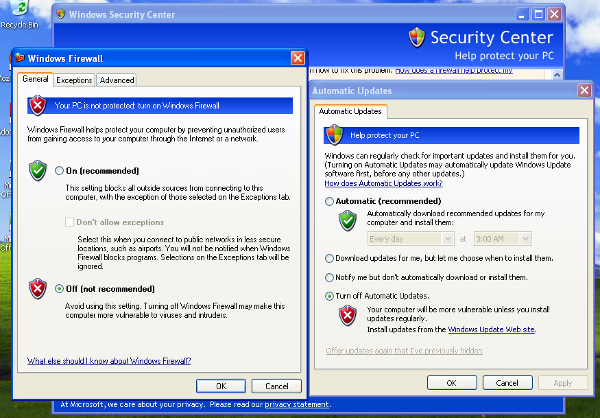
\includegraphics{windows_security.png}
\end{figure}
\end{quote}


\paragraph{Virtual Networking}
\label{installation/guest/network:virtual-networking}
Now you need to decide how to make your virtual machine able to access Internet
or your local network.

By default VirtualBox adopts Network Address Translation (NAT) which in most
cases will be good enough for any needs.
This is also the configuration we'll adopt in this documentation.

If you have particular needs and want to use some different networking, please
refer to VirtualBox's \href{https://www.virtualbox.org/manual/ch06.html}{virtual networking documentation}.


\paragraph{Network Tracing}
\label{installation/guest/network:network-tracing}\label{installation/guest/network:virtual-networking-documentation}
Unless you decided to use an external sniffer (as previously discussed in
{\hyperref[installation/host/configuration::doc]{\emph{Configuration}}}), you can proceed configuring the network trace
functionality provided by VirtualBox as explained \href{https://www.virtualbox.org/wiki/Network\_tips}{here}.

First you need to power off your virtual machine:

\begin{Verbatim}[commandchars=@\[\]]
@$ VBoxManage controlvm "Name of VM" poweroff
\end{Verbatim}

Then you enable network trace:

\begin{Verbatim}[commandchars=@\[\]]
@$ VBoxManage modifyvm "Name of VM" --nictrace1 on --nictracefile1 /path/to/cuckoo/shares/@textless[]VM ID@textgreater[]/dump.pcap
\end{Verbatim}

The last argument specifies the path where the PCAP file will be stored. It has
to be an absolute path and include the file name as well. In order to make
Cuckoo able to find the file you'll have to specify the shared folder you
created for current virtual machine and ``\emph{dump.pcap}''.


\subsubsection{Shared Folders}
\label{installation/guest/shares:shared-folders}\label{installation/guest/shares::doc}\label{installation/guest/shares:here}
Cuckoo exchanges data between the host and the guest using VirtualBox's Shared
Folders.

In order to have them enabled on your virtual machine you should have installed
the Guest Additions as specified in {\hyperref[installation/guest/requirements::doc]{\emph{Requirements}}}.

You will have to add two shared folders:
\begin{itemize}
\item {} 
\textbf{shares/setup}: which is used to get Cuckoo analyzer's components to be run inside virtualized Windows.

\item {} 
\textbf{shares/\textless{}VM ID\textgreater{}}: the unique shared folder associated with your current Virtual Machine, which is used to store the analysis results.

\end{itemize}

You can do so from VirtualBox's graphical user interface or from the command line:

\begin{Verbatim}[commandchars=@\[\]]
@$ VBoxManage sharedfolder add "@textless[]Name of VM@textgreater[]" --name "setup" --hostpath "/path/to/cuckoo/shares/setup" --readonly
@$ VBoxManage sharedfolder add "@textless[]Name of VM@textgreater[]" --name "@textless[]VM ID@textgreater[]" --hostpath "/path/to/cuckoo/shares/@textless[]VM ID@textgreater[]"
\end{Verbatim}

Where ``\emph{\textless{}Name of VM\textgreater{}}'' is the label you gave to the virtual machine in VirtualBox
and ``\emph{\textless{}VM ID\textgreater{}}'' is the ID you assigned to the Virtual Machine in Cuckoo.

Using the GUI, you should see something similar to this:
\begin{quote}
\begin{figure}[htbp]
\centering

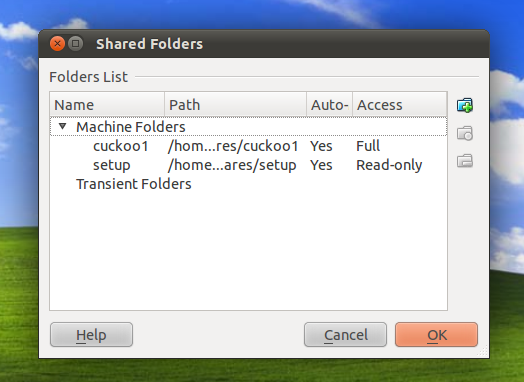
\includegraphics{shared_folders.png}
\end{figure}
\end{quote}


\subsubsection{Saving the Virtual Machine}
\label{installation/guest/saving:saving-the-virtual-machine}\label{installation/guest/saving::doc}
Now you should be ready to go and save the virtual machine to a snapshot state.

Before doing this make sure you rebooted it softly and that it's currently
running and with your Windows user logged in. Once you are sure that the
operating system is fully booted and ready to be snapshotted you can proceed.

You can take the snapshot from the graphical user interface or from the command
line:

\begin{Verbatim}[commandchars=@\[\]]
@$ VBoxManage snapshot "@textless[]Name of VM@textgreater[]" take "@textless[]Name of snapshot@textgreater[]" --pause
\end{Verbatim}

After the snapshot creation is completed, you can power off the machine and
restore it:

\begin{Verbatim}[commandchars=@\[\]]
@$ VBoxManage controlvm "@textless[]Name of VM@textgreater[]" poweroff
@$ VBoxManage snapshot "@textless[]Name of VM"@textgreater[] restorecurrent
\end{Verbatim}

If you followed all the steps properly, your virtual machine should be ready to
be used by Cuckoo.


\subsubsection{Cloning the Virtual Machine}
\label{installation/guest/cloning:cloning-the-virtual-machine}\label{installation/guest/cloning::doc}
In case you planned to use more than one virtual machine, there's no need to
repeat all the steps done so far: you can clone it. In this way you'll have
a copy of the original virtualized Windows with all requirements already
installed.

To clone a machine you can use the graphical user interface (at least in the
most recent versions of VirtualBox) or from the command line:

\begin{Verbatim}[commandchars=@\[\]]
@$ VBoxManage clonevm "@textless[]Name of original VM@textgreater[]" --name "@textless[]Name of new VM@textgreater[]" --registervm
\end{Verbatim}

Now you have an exact copy of your original virtual machine saved with the new
name you specified.

Obviously the new virtual machine will bring along also the settings of the
original one, which is not good. Now you need to proceed repeating the steps
explained in {\hyperref[installation/guest/network::doc]{\emph{Network Configuration}}}, {\hyperref[installation/guest/shares::doc]{\emph{Shared Folders}}} and {\hyperref[installation/guest/saving::doc]{\emph{Saving the Virtual Machine}}} for this new
machine.


\section{Usage}
\label{usage/index:usage}\label{usage/index::doc}
This chapter explains how to use Cuckoo.


\subsection{Starting Cuckoo}
\label{usage/start::doc}\label{usage/start:starting-cuckoo}
To start Cuckoo use the command:

\begin{Verbatim}[commandchars=@\[\]]
@$ python cuckoo.py
\end{Verbatim}

Make sure to run it inside Cuckoo's root directory.

You will get an output similar to this:

\begin{Verbatim}[commandchars=@\[\]]
                     @_
    @_@_@_@_ @_   @_  @_@_@_@_@textbar[] @textbar[]  @_ @_@_@_   @_@_@_
   / @_@_@_) @textbar[] @textbar[] @textbar[]/ @_@_@_) @textbar[]@_/ ) @_ \ / @_ \
  ( (@_@_@_@textbar[] @textbar[]@_@textbar[] ( (@_@_@_@textbar[]  @_ ( @textbar[]@_@textbar[] @textbar[] @textbar[]@_@textbar[] @textbar[]
   \@_@_@_@_)@_@_@_@_/ \@_@_@_@_)@_@textbar[] \@_)@_@_@_/ \@_@_@_/ v0.3

 www.cuckoobox.org
 Copyright (C) 2010-2011

@PYGZlb[]2011-12-18 17:43:06,343@PYGZrb[] @PYGZlb[]Core.Init@PYGZrb[] INFO: Started.
@PYGZlb[]2011-12-18 17:43:06,834@PYGZrb[] @PYGZlb[]VirtualMachine.Check@PYGZrb[] INFO: Your VirtualBox version is: "4.1.6", good!
@PYGZlb[]2011-12-18 17:43:06,834@PYGZrb[] @PYGZlb[]Core.Init@PYGZrb[] INFO: Populating virtual machines pool...
@PYGZlb[]2011-12-18 17:43:06,840@PYGZrb[] @PYGZlb[]VirtualMachine.Infos@PYGZrb[] INFO: Virtual machine "Cuckoo1" information:
@PYGZlb[]2011-12-18 17:43:06,841@PYGZrb[] @PYGZlb[]VirtualMachine.Infos@PYGZrb[] INFO:      \@_@textbar[] Name: Cuckoo1
@PYGZlb[]2011-12-18 17:43:06,841@PYGZrb[] @PYGZlb[]VirtualMachine.Infos@PYGZrb[] INFO:        @textbar[] ID: xxxxxxxx-xxxx-xxxx-xxxx-xxxxxxxxxxxx
@PYGZlb[]2011-12-18 17:43:06,841@PYGZrb[] @PYGZlb[]VirtualMachine.Infos@PYGZrb[] INFO:        @textbar[] CPU Count: 1 Core/s
@PYGZlb[]2011-12-18 17:43:06,841@PYGZrb[] @PYGZlb[]VirtualMachine.Infos@PYGZrb[] INFO:        @textbar[] Memory Size: 192 MB
@PYGZlb[]2011-12-18 17:43:06,841@PYGZrb[] @PYGZlb[]VirtualMachine.Infos@PYGZrb[] INFO:        @textbar[] VRAM Size: 16 MB
@PYGZlb[]2011-12-18 17:43:06,841@PYGZrb[] @PYGZlb[]VirtualMachine.Infos@PYGZrb[] INFO:        @textbar[] State: Saved
@PYGZlb[]2011-12-18 17:43:06,842@PYGZrb[] @PYGZlb[]VirtualMachine.Infos@PYGZrb[] INFO:        @textbar[] Current Snapshot: "Clean"
@PYGZlb[]2011-12-18 17:43:06,842@PYGZrb[] @PYGZlb[]VirtualMachine.Infos@PYGZrb[] INFO:        @textbar[] MAC Address: 08:00:27:XX:XX:XX
@PYGZlb[]2011-12-18 17:43:06,842@PYGZrb[] @PYGZlb[]Core.Init@PYGZrb[] INFO: 1 virtual machine/s added to pool.
@PYGZlb[]2011-12-18 17:43:07,045@PYGZrb[] @PYGZlb[]Database.Init@PYGZrb[] INFO: Generated database "db/cuckoo.db" which didn't exist before.
\end{Verbatim}

Now Cuckoo is ready to run and it's listening for submissions.


\subsection{Submit an analysis}
\label{usage/submit::doc}\label{usage/submit:submit-an-analysis}
In order to submit a file to be analyzed you can:
\begin{itemize}
\item {} 
Use provided \textbf{submit.py} utility.

\item {} 
Directly interact with the \textbf{SQLite database}.

\item {} 
Use Cuckoo \textbf{Python functions} directly from Cuckoo's library.

\end{itemize}


\subsubsection{Submission Utility}
\label{usage/submit:submission-utility}
The easiest way to submit an analysis is to use the provided \emph{submit.py}
command-line utility. It currently has the following options available:

\begin{Verbatim}[commandchars=@\[\]]
Usage: submit.py @PYGZlb[]options@PYGZrb[] filepath

Options:
  -h, --help            show this help message and exit
  -t TIMEOUT, --timeout=TIMEOUT
                        Specify analysis execution time limit
  -p PACKAGE, --package=PACKAGE
                        Specify custom analysis package name
  -r PRIORITY, --priority=PRIORITY
                        Specify an analysis priority expressed in integer
  -c CUSTOM, --custom=CUSTOM
                        Specify any custom value to be passed to postprocessing
  -d, --download        Specify if the target is an URL to be downloaded
  -u, --url             Specify if the target is an URL to be analyzed
  -m MACHINE, --machine=MACHINE
                        Specify a virtual machine you want to specifically use for this analysis
\end{Verbatim}

The concept of analysis packages will be dealt later in this documentation (at
{\hyperref[usage/packages::doc]{\emph{Analysis Packages}}}). Following are some usage examples:

\textbf{Example}: submit a local binary:

\begin{Verbatim}[commandchars=@\[\]]
@$ python submit.py /path/to/binary
\end{Verbatim}

\textbf{Example}: submit a local binary and specify an higher priority:

\begin{Verbatim}[commandchars=@\[\]]
@$ python submit.py /path/to/binary --priority 5
\end{Verbatim}

\textbf{Example}: submit a local binary and specify a custom analysis timeout of
60 seconds:

\begin{Verbatim}[commandchars=@\[\]]
@$ python submit.py /path/to/binary --timeout 60
\end{Verbatim}

\textbf{Example}: submit a local binary and specify a custom analysis package:

\begin{Verbatim}[commandchars=@\[\]]
@$ python submit.py /path/to/binary --package @textless[]name of package@textgreater[]
\end{Verbatim}

\textbf{Example}: submit an URL to be downloaded locally and analyzed:

\begin{Verbatim}[commandchars=@\[\]]
@$ python submit.py --download http://www.website.tld/file.exe
\end{Verbatim}

\textbf{Example}: submit an URL to be analyzed within Internet Explorer:

\begin{Verbatim}[commandchars=@\[\]]
@$ python submit.py --url http://maliciousurl.tld/exploit.php
\end{Verbatim}

\textbf{Example}: submit a local binary to be run on virtual machine \emph{cuckoo1}:

\begin{Verbatim}[commandchars=@\[\]]
@$ python submit.py /path/to/binary --machine cuckoo1
\end{Verbatim}


\subsubsection{Interact with SQLite}
\label{usage/submit:interact-with-sqlite}
Cuckoo is designed to be easily integrated in larger solutions and to be fully
automated. In order to automate analysis submission or to provide a different
interface rather than the command-line (for instance a web interface), you can
directly interact with the SQLite database located at \emph{db/cuckoo.db}.

The database contains the table \emph{queue} which is defined as the following schema:
\begin{quote}

\begin{Verbatim}[commandchars=\\\{\},numbers=left,firstnumber=1,stepnumber=1]
\PYG{k}{CREATE} \PYG{k}{TABLE} \PYG{n}{queue} \PYG{p}{(}
  \PYG{n}{id} \PYG{n+nb}{INTEGER} \PYG{k}{PRIMARY} \PYG{k}{KEY}\PYG{p}{,}
  \PYG{n}{md5} \PYG{n+nb}{TEXT} \PYG{k}{DEFAULT} \PYG{k}{NULL}\PYG{p}{,}
  \PYG{n}{target} \PYG{n+nb}{TEXT} \PYG{k}{NOT} \PYG{k}{NULL}\PYG{p}{,}
  \PYG{n}{timeout} \PYG{n+nb}{INTEGER} \PYG{k}{DEFAULT} \PYG{k}{NULL}\PYG{p}{,}
  \PYG{n}{priority} \PYG{n+nb}{INTEGER} \PYG{k}{DEFAULT} \PYG{l+m+mi}{0}\PYG{p}{,}
  \PYG{n}{added\PYGZus{}on} \PYG{n+nb}{DATE} \PYG{k}{DEFAULT} \PYG{k}{CURRENT\PYGZus{}TIMESTAMP}\PYG{p}{,}
  \PYG{n}{completed\PYGZus{}on} \PYG{n+nb}{DATE} \PYG{k}{DEFAULT} \PYG{k}{NULL}\PYG{p}{,}
  \PYG{n}{package} \PYG{n+nb}{TEXT} \PYG{k}{DEFAULT} \PYG{k}{NULL}\PYG{p}{,}
  \PYG{k}{lock} \PYG{n+nb}{INTEGER} \PYG{k}{DEFAULT} \PYG{l+m+mi}{0}\PYG{p}{,}
  \PYG{n}{status} \PYG{n+nb}{INTEGER} \PYG{k}{DEFAULT} \PYG{l+m+mi}{0}\PYG{p}{,}
  \PYG{n}{custom} \PYG{n+nb}{TEXT} \PYG{k}{DEFAULT} \PYG{k}{NULL}\PYG{p}{,}
  \PYG{n}{vm\PYGZus{}id} \PYG{n+nb}{TEXT} \PYG{k}{DEFAULT} \PYG{k}{NULL}
\PYG{p}{)}\PYG{p}{;}
\end{Verbatim}
\end{quote}

Following are the details on the fields:
\begin{itemize}
\item {} 
\code{id}: it's the numeric ID also used to name the results folder of the analysis.

\item {} 
\code{md5}: it's the MD5 hash of the target file.

\item {} 
\code{target}: it's the path pointing to the file to analyze.

\item {} 
\code{timeout}: it's the analysis timeout, if none has been specified the field is set to NULL.

\item {} 
\code{priority}: it's the analysis priority, if none has been specified the field is set to NULL.

\item {} 
\code{added\_on}: it's the timestamp of when the analysis request was added.

\item {} 
\code{completed\_on}: it's the timestamp of when the analysis has been completed.

\item {} 
\code{package}: it's the name of the analysis package to be used, if non has been specified the field is set to NULL.

\item {} 
\code{lock}: it's field internally used by Cuckoo to lock pending analysis.

\item {} 
\code{status}: it's a numeric field representing the status of the analysis (0 = not completed, 1 = completed successfully, 2 = failed).

\item {} 
\code{custom}: it's a custom user-defined text that can be used for synchronization between submission and post-analysis processing.

\item {} 
\code{vm\_id}: it's the ID (as defined in cuckoo.conf) of a virtual machine the user specifically wants to use for the analysis.

\end{itemize}


\subsubsection{Cuckoo Python Functions}
\label{usage/submit:cuckoo-python-functions}
In case you want to write your own Python submission script, you can use the
\code{add\_task()} function provided by Cuckoo, which has the following prototype:
\begin{quote}

\begin{Verbatim}[commandchars=@\[\]]
def add@_task(self, target, md5 = None, timeout = None, package = None, priority = None, custom = None, vm@_id = None)
\end{Verbatim}
\end{quote}

Following is a usage example:
\begin{quote}

\begin{Verbatim}[commandchars=\\\{\},numbers=left,firstnumber=1,stepnumber=1]
\PYG{c}{\PYGZsh{}!/usr/bin/python}
\PYG{k+kn}{from} \PYG{n+nn}{cuckoo.core.db} \PYG{k+kn}{import} \PYG{n}{CuckooDatabase}

\PYG{n}{db} \PYG{o}{=} \PYG{n}{CuckooDatabase}\PYG{p}{(}\PYG{p}{)}
\PYG{n}{db}\PYG{o}{.}\PYG{n}{add\PYGZus{}task}\PYG{p}{(}\PYG{l+s}{"}\PYG{l+s}{/path/to/binary}\PYG{l+s}{"}\PYG{p}{)}
\end{Verbatim}
\end{quote}


\subsection{Analysis Packages}
\label{usage/packages:analysis-packages}\label{usage/packages::doc}
The \textbf{analysis packages} are a key component in Cuckoo Sandbox.

They consist in structured Python scripts which are executed inside the virtual
machine and that define how Cuckoo should conduct the analysis.

As you already know, you can choose which analysis package to use by specifying
its name at submission time (see {\hyperref[usage/submit::doc]{\emph{Submit an analysis}}}) like following:

\begin{Verbatim}[commandchars=@\[\]]
@$ python submit.py /path/to/malware --package @textless[]package name@textgreater[]
\end{Verbatim}

If none is specified, Cuckoo will try to detect the type of the file and choose
the proper analysis package accordingly. If the file type is not supported and
no package was specified, the analysis will be aborted and marked as failed in
the database.

This functionality allows you not only to use existing analysis packages, but
also create some of your own and customize your Cuckoo setup. Ths topic will
be dealt in details in the {\hyperref[customization/packages::doc]{\emph{Analysis Packages}}} customization
chapter.

Cuckoo provides some default analysis packages which include:
\begin{itemize}
\item {} 
\code{exe}: default analysis package used to analyze generic Windows executables.

\item {} 
\code{dll}: used to analyze Dynamic Linked Libraries.

\item {} 
\code{pdf}: used to analyze Adobe Reader while opening the given PDF file.

\item {} 
\code{doc}: used to analyze Microsoft Office while opening documents.

\item {} 
\code{php}: used to analyze PHP scripts.

\item {} 
\code{ie}: used to analyze Internet Explorer while opening the given URL.

\item {} 
\code{firefox}: used to analyze Mozilla Firefox while opening the given URL.

\item {} 
\code{tracer}: used to trace assembly instructions performed by the given file.

\end{itemize}


\subsection{Execution}
\label{usage/execution:execution}\label{usage/execution::doc}
When Cuckoo receives an analysis request, you'll see something like this:
\begin{quote}

\begin{Verbatim}[commandchars=\\\{\},numbers=left,firstnumber=1,stepnumber=1]
[2011-12-18 18:20:16,242] [Core.Dispatcher] INFO: Acquired analysis task for target "/tmp/malware.exe".
[2011-12-18 18:20:16,424] (Task \PYGZsh{}1) [Core.Analysis.Run] INFO: Acquired virtual machine "cuckoo1".
[2011-12-18 18:20:17,005] [VirtualMachine.Restore] INFO: Virtual machine "Cuckoo1" successfully restored to current snapshot.
[2011-12-18 18:20:19,779] [VirtualMachine.Start] INFO: Virtual machine "Cuckoo1" starting in "gui" mode.
[2011-12-18 18:20:24,429] [VirtualMachine.Execute] INFO: Cuckoo analyzer running with PID 1732 on virtual machine "Cuckoo1".
[2011-12-18 18:20:54,871] [VirtualMachine.Execute] INFO: Cuckoo analyzer exited with code 0 on virtual machine "Cuckoo1".
[2011-12-18 18:20:54,878] (Task \PYGZsh{}1) [Core.Analysis.SaveResults] INFO: Analysis results successfully saved to "analysis/1".
[2011-12-18 18:20:55,124] (Task \PYGZsh{}1) [Core.Analysis.Processing] INFO: Analysis results processor started with PID "8571".
[2011-12-18 18:20:56,307] [VirtualMachine.Stop] INFO: Virtual machine "Cuckoo1" powered off successfully.
[2011-12-18 18:20:56,308] (Task \PYGZsh{}1) [Core.Analysis.FreeVM] INFO: Virtual machine "cuckoo1" released.
[2011-12-18 18:20:56,309] (Task \PYGZsh{}1) [Core.Analysis.Run] INFO: Analyis completed.
\end{Verbatim}
\end{quote}

Let's get through what happened.

At line \textbf{1} Cuckoo's tasks dispatcher acquired a new submission for the target
\emph{/tmp/malware.exe}. At line \textbf{2} it acquired the free virtual machine \emph{cuckoo1}.
At line \textbf{3} Cuckoo restored the virtual machine to current snapshot and at
line \textbf{4} it started it in graphical mode.

In the meanwhile it prepared all required files and configurations for the
analysis.

At line \textbf{5} Cuckoo analyzer component started inside the virtualized Windows
environment with process ID \emph{1732}. At line \textbf{6}, after the 60 seconds of the
specified timeout, the analyzer terminates its execution and exits. At line
\textbf{7} the analysis results are stored to \emph{analysis/1/} and this same path is
specified to the processor script which is invoked at line \textbf{8} with process ID
\emph{8571}. At line \textbf{9} the virtual machine is successfully powered off and
released at line \textbf{10}. At line \textbf{11} finally Cuckoo considers the analysis as
completed.

At this point you should have complete analysis results into \emph{analysis/1/} and,
depending on the options you enabled in \emph{reporting.conf}
({\hyperref[installation/host/configuration::doc]{\emph{Configuration}}}), some automatically generated
reports at \emph{analysis/1/reports/}.


\subsection{Analysis Results}
\label{usage/results::doc}\label{usage/results:analysis-results}
Once an analysis is completed, several files are stored in a dedicated directory.
Unless you configured differently, all of the analysis are saved into
\emph{analysis/} with a subdirectory named after the numerical ID assigned to the
analysis into the database.

Following is an example of analysis results:

\begin{Verbatim}[commandchars=@\[\]]
.
@textbar[]-- analysis.conf
@textbar[]-- analysis.log
@textbar[]-- dump.pcap
@textbar[]-- files
@textbar[]   @textbar[]-- dropped.tmp
@textbar[]   []`-- dropped.exe
@textbar[]-- logs
@textbar[]   @textbar[]-- 1232.csv
@textbar[]   @textbar[]-- 1540.csv
@textbar[]   []`-- 1118.csv
@textbar[]-- reports
@textbar[]   @textbar[]-- report.html
@textbar[]   @textbar[]-- report.json
@textbar[]   []`-- report.txt
@textbar[]-- malware.exe
@textbar[]-- shots
@textbar[]   @textbar[]-- shot@_1.jpg
@textbar[]   @textbar[]-- shot@_2.jpg
@textbar[]   @textbar[]-- shot@_3.jpg
@textbar[]   []`-- shot@_4.jpg
[]`-- trace
\end{Verbatim}


\subsubsection{analysis.conf}
\label{usage/results:analysis-conf}
\emph{analysis.conf} is a configuration file automatically generated by Cuckoo to
specify some parameters to the guest component (analyzer).
It's generally not relevant for an end-users as it's exclusively used internally
by Cuckoo.


\subsubsection{analysis.log}
\label{usage/results:analysis-log}
\emph{analysis.log} is a log file generated by Cuckoo analyzer and that keeps
track of analysis execution and might report errors occurred during the
analysis.


\subsubsection{dump.pcap}
\label{usage/results:dump-pcap}
\emph{dump.pcap} is the trace dump containing all the network activity generated by
the virtual machine during the malware execution.


\subsubsection{files/}
\label{usage/results:files}
The \emph{files/} directory contains all files created or deleted by the malware and
that were successfully dumped by Cuckoo.


\subsubsection{logs/}
\label{usage/results:logs}
The \emph{logs/} directory contains the raw CSV-like logs generated by the monitored
processes and that contains the concrete behavioral tracing results.


\subsubsection{reports/}
\label{usage/results:reports}
The \emph{reports/} directory contains the abstract analysis reports generated
automatically by Cuckoo. The number and the format of such reports depends on
the the configuration explained in the {\hyperref[installation/host/configuration::doc]{\emph{Configuration}}}
chapter.


\subsubsection{shots/}
\label{usage/results:shots}
The \emph{shots/} directory contains the screenshots of Windows desktop taken during
the analysis execution.


\subsubsection{trace/}
\label{usage/results:trace}
The \emph{trace/} directory is only used in specific cases (for instance when using
the \emph{tracer} analysis package) and contains the assembly instruction traces of
the monitored processes.


\subsection{Web Interface}
\label{usage/web:web-interface}\label{usage/web::doc}
Cuckoo Sandbox comes with a very simple and handy web server which is used
to navigate and view analysis reports.


\subsubsection{Start the Web Server}
\label{usage/web:start-the-web-server}
The web server has following options:

\begin{Verbatim}[commandchars=@\[\]]
Usage: web.py @PYGZlb[]options@PYGZrb[]

Options:
  -h, --help            show this help message and exit
  -t HOST, --host=HOST  Specify the host to bind the server on (default localhost)
  -p PORT, --port=PORT  Specify the port to bind the server on (default 8080)
\end{Verbatim}

In order to start it, just launch:

\begin{Verbatim}[commandchars=@\[\]]
@$ python web.py
\end{Verbatim}

You should see displayed:

\begin{Verbatim}[commandchars=@\[\]]
Starting web server on localhost:8080
\end{Verbatim}

You can change the host and the port on which to bind the web server by
specifying them with the appropriate options.


\subsubsection{Recent Analysis}
\label{usage/web:recent-analysis}
If you now open your browser and go to \emph{http://localhost:8080/} you will see
Cuckoo's index page, which includes a list of the 30 most recent analysis and
a web form through which you can search for analysis by MD5 hash.
\begin{quote}
\begin{figure}[htbp]
\centering

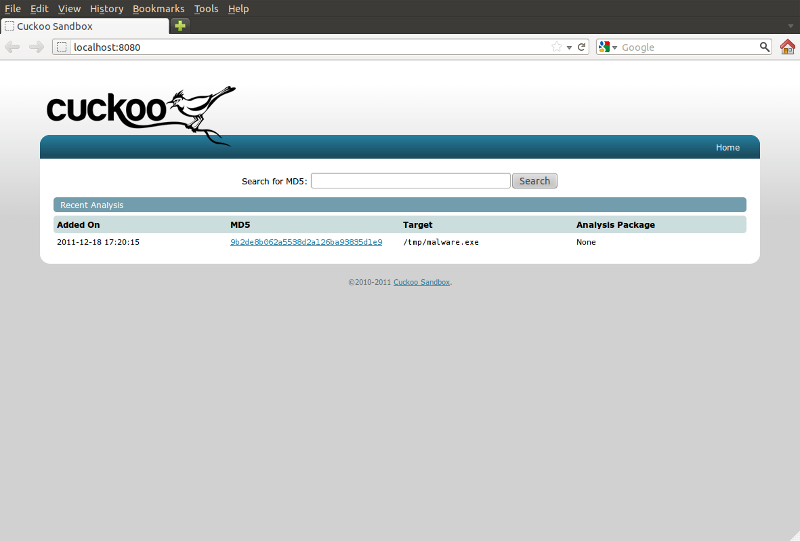
\includegraphics{cuckoo_web_index.png}
\end{figure}
\end{quote}

By filling the form and submitting it you'll be prompted with search results.
By clicking on the MD5 of one of the analysis, you'll be prompted with the
report for that specific analysis.


\subsubsection{Search for MD5}
\label{usage/web:search-for-md5}
After submitting a valid MD5 in the search form, you'll be prompted with all the
analysis performed on the file matching that hash.
\begin{quote}
\begin{figure}[htbp]
\centering

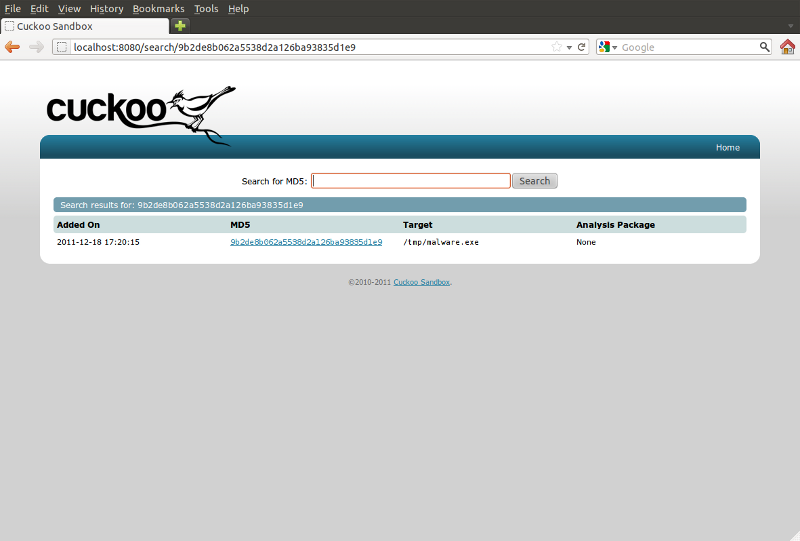
\includegraphics{cuckoo_web_search.png}
\end{figure}
\end{quote}


\subsubsection{View Report}
\label{usage/web:view-report}
When requesting the report of a specific analysis, the web server will returns
you the appropriate HTML report. Please notice that if in your Cuckoo Setup
you disabled the generation of HTML reports (see {\hyperref[installation/host/configuration::doc]{\emph{Configuration}}}),
a 404 error will be returned.
\begin{quote}
\begin{figure}[htbp]
\centering

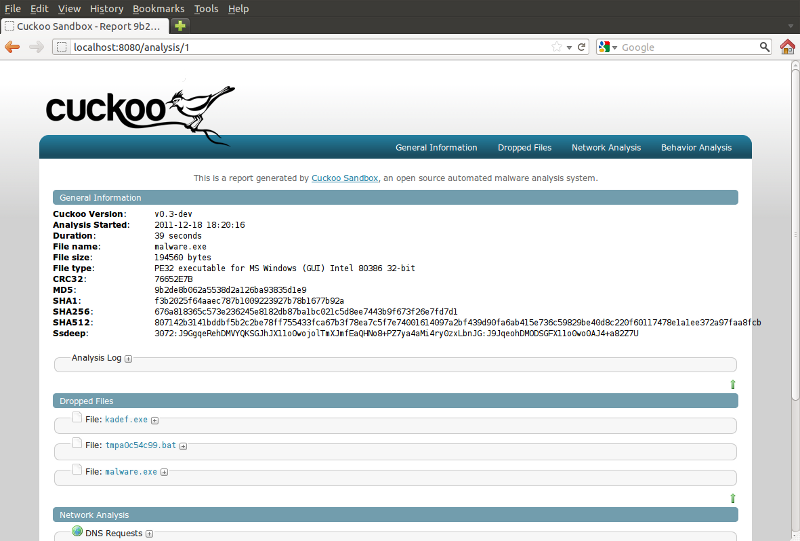
\includegraphics{cuckoo_web_analysis.png}
\end{figure}
\end{quote}


\section{Customization}
\label{customization/index::doc}\label{customization/index:customization}
This chapter explains how to customize Cuckoo.
Cuckoo is written in a modular architecture built to be as much customizable it can,
to fit all user's needs.


\subsection{Analysis Packages}
\label{customization/packages:analysis-packages}\label{customization/packages::doc}
As explained in {\hyperref[usage/packages::doc]{\emph{Analysis Packages}}}, analysis packages are structured
Python scripts that allow you to customize the analysis procedure inside the
virtualized Windows environment.

By default Cuckoo provides some default packages you can already use, but you
are able to create and use some of your own.

Creating new packages is really easy and just requires minimal knowledge of the
Python language.


\subsubsection{Getting started}
\label{customization/packages:getting-started}
As first example we'll take a look at the default package for analyzing generic
Windows executables (located at \emph{shares/setup/packages/exe.py}):
\begin{quote}

\begin{Verbatim}[commandchars=\\\{\},numbers=left,firstnumber=1,stepnumber=1]
\PYG{k+kn}{import} \PYG{n+nn}{os}
\PYG{k+kn}{import} \PYG{n+nn}{sys}

\PYG{n}{sys}\PYG{o}{.}\PYG{n}{path}\PYG{o}{.}\PYG{n}{append}\PYG{p}{(}\PYG{l+s}{"}\PYG{l+s+se}{\PYGZbs{}\PYGZbs{}}\PYG{l+s+se}{\PYGZbs{}\PYGZbs{}}\PYG{l+s}{VBOXSVR}\PYG{l+s+se}{\PYGZbs{}\PYGZbs{}}\PYG{l+s}{setup}\PYG{l+s+se}{\PYGZbs{}\PYGZbs{}}\PYG{l+s}{lib}\PYG{l+s+se}{\PYGZbs{}\PYGZbs{}}\PYG{l+s}{"}\PYG{p}{)}

\PYG{k+kn}{from} \PYG{n+nn}{cuckoo.execute} \PYG{k+kn}{import} \PYG{n}{cuckoo\PYGZus{}execute}
\PYG{k+kn}{from} \PYG{n+nn}{cuckoo.monitor} \PYG{k+kn}{import} \PYG{n}{cuckoo\PYGZus{}monitor}

\PYG{c}{\PYGZsh{} The package main function "cuckoo\PYGZus{}run" should follow a fixed structure in}
\PYG{c}{\PYGZsh{} order for Cuckoo to correctly handle it and its results.}
\PYG{k}{def} \PYG{n+nf}{cuckoo\PYGZus{}run}\PYG{p}{(}\PYG{n}{target\PYGZus{}path}\PYG{p}{)}\PYG{p}{:}
    \PYG{c}{\PYGZsh{} Every analysis package can retrieve a list of multiple process IDs it}
    \PYG{c}{\PYGZsh{} might have generated. All processes added to this list will be added to}
    \PYG{c}{\PYGZsh{} the monitored list, and Cuckoo will wait for all of the to complete their}
    \PYG{c}{\PYGZsh{} execution before ending the analysis.}
    \PYG{n}{pids} \PYG{o}{=} \PYG{p}{[}\PYG{p}{]}

    \PYG{c}{\PYGZsh{} The following functions are used to launch a process with the simplified}
    \PYG{c}{\PYGZsh{} "cuckoo\PYGZus{}execute" function. This function takes as arguments (in specific}
    \PYG{c}{\PYGZsh{} order):}
    \PYG{c}{\PYGZsh{} - a path to the executable to launch}
    \PYG{c}{\PYGZsh{} - arguments to be passed on execution}
    \PYG{c}{\PYGZsh{} - a boolean value to specify if the process have to be created in}
    \PYG{c}{\PYGZsh{}   suspended mode or not (it's recommended to set it to True if the}
    \PYG{c}{\PYGZsh{}   process is supposed to be injected and monitored).}
    \PYG{n}{suspended} \PYG{o}{=} \PYG{n+nb+bp}{True}
    \PYG{p}{(}\PYG{n}{pid}\PYG{p}{,} \PYG{n}{h\PYGZus{}thread}\PYG{p}{)} \PYG{o}{=} \PYG{n}{cuckoo\PYGZus{}execute}\PYG{p}{(}\PYG{n}{target\PYGZus{}path}\PYG{p}{,} \PYG{n+nb+bp}{None}\PYG{p}{,} \PYG{n}{suspended}\PYG{p}{)}

    \PYG{c}{\PYGZsh{} The function "cuckoo\PYGZus{}monitor" invoke the DLL injection and resume the}
    \PYG{c}{\PYGZsh{} process if it was suspended. It needs the process id and the main thread}
    \PYG{c}{\PYGZsh{} handle returned by "cuckoo\PYGZus{}execute" and the same boolean value to tell it}
    \PYG{c}{\PYGZsh{} if it needs to resume the process.}
    \PYG{n}{cuckoo\PYGZus{}monitor}\PYG{p}{(}\PYG{n}{pid}\PYG{p}{,} \PYG{n}{h\PYGZus{}thread}\PYG{p}{,} \PYG{n}{suspended}\PYG{p}{)}

    \PYG{c}{\PYGZsh{} Append all the process IDs you want to the list, and return the list.}
    \PYG{n}{pids}\PYG{o}{.}\PYG{n}{append}\PYG{p}{(}\PYG{n}{pid}\PYG{p}{)}
    \PYG{k}{return} \PYG{n}{pids}

\PYG{k}{def} \PYG{n+nf}{cuckoo\PYGZus{}check}\PYG{p}{(}\PYG{p}{)}\PYG{p}{:}
    \PYG{k}{return} \PYG{n+nb+bp}{True}

\PYG{k}{def} \PYG{n+nf}{cuckoo\PYGZus{}finish}\PYG{p}{(}\PYG{p}{)}\PYG{p}{:}
    \PYG{k}{return} \PYG{n+nb+bp}{True}
\end{Verbatim}
\end{quote}

Let's walk through the given code.

At line \textbf{1} and \textbf{2} we import the \code{os} and \code{sys} Python modules.
At line \textbf{4} we append ``\emph{\textbackslash{}\textbackslash{}VBOXSVR\textbackslash{}setup\textbackslash{}lib\textbackslash{}}'' to Python's modules paths list:
this will allow us to invoke Cuckoo's modules directly from the shared folder.

Then we can see that three functions are defined:
\begin{itemize}
\item {} 
{\hyperref[customization/packages:cuckoo-run]{\emph{cuckoo\_run()}}}

\item {} 
{\hyperref[customization/packages:cuckoo-check]{\emph{cuckoo\_check()}}}

\item {} 
{\hyperref[customization/packages:cuckoo-finish]{\emph{cuckoo\_finish()}}}

\end{itemize}

In the given example the package just executes the binary located at \code{target\_path}
in suspended mode and instructs Cuckoo to inject the process and start
monitoring it.

A slightly more complex example is the PDF analysis package (located at
\emph{shares/setup/packages/pdf.py}):
\begin{quote}

\begin{Verbatim}[commandchars=\\\{\},numbers=left,firstnumber=1,stepnumber=1]
\PYG{k+kn}{import} \PYG{n+nn}{os}
\PYG{k+kn}{import} \PYG{n+nn}{sys}

\PYG{n}{sys}\PYG{o}{.}\PYG{n}{path}\PYG{o}{.}\PYG{n}{append}\PYG{p}{(}\PYG{l+s}{"}\PYG{l+s+se}{\PYGZbs{}\PYGZbs{}}\PYG{l+s+se}{\PYGZbs{}\PYGZbs{}}\PYG{l+s}{VBOXSVR}\PYG{l+s+se}{\PYGZbs{}\PYGZbs{}}\PYG{l+s}{setup}\PYG{l+s+se}{\PYGZbs{}\PYGZbs{}}\PYG{l+s}{lib}\PYG{l+s+se}{\PYGZbs{}\PYGZbs{}}\PYG{l+s}{"}\PYG{p}{)}

\PYG{k+kn}{from} \PYG{n+nn}{cuckoo.execute} \PYG{k+kn}{import} \PYG{n}{cuckoo\PYGZus{}execute}
\PYG{k+kn}{from} \PYG{n+nn}{cuckoo.monitor} \PYG{k+kn}{import} \PYG{n}{cuckoo\PYGZus{}monitor}

\PYG{k}{def} \PYG{n+nf}{cuckoo\PYGZus{}run}\PYG{p}{(}\PYG{n}{target\PYGZus{}path}\PYG{p}{)}\PYG{p}{:}
    \PYG{n}{pids} \PYG{o}{=} \PYG{p}{[}\PYG{p}{]}

    \PYG{c}{\PYGZsh{} Customize this Path with the correct one on your Windows setup.}
    \PYG{n}{adobe\PYGZus{}reader} \PYG{o}{=} \PYG{l+s}{"}\PYG{l+s}{C:}\PYG{l+s+se}{\PYGZbs{}\PYGZbs{}}\PYG{l+s}{Program Files}\PYG{l+s+se}{\PYGZbs{}\PYGZbs{}}\PYG{l+s}{Adobe}\PYG{l+s+se}{\PYGZbs{}\PYGZbs{}}\PYG{l+s}{Reader 9.0}\PYG{l+s+se}{\PYGZbs{}\PYGZbs{}}\PYG{l+s}{Reader}\PYG{l+s+se}{\PYGZbs{}\PYGZbs{}}\PYG{l+s}{AcroRd32.exe}\PYG{l+s}{"}

    \PYG{n}{suspended} \PYG{o}{=} \PYG{n+nb+bp}{True}
    \PYG{p}{(}\PYG{n}{pid}\PYG{p}{,} \PYG{n}{h\PYGZus{}thread}\PYG{p}{)} \PYG{o}{=} \PYG{n}{cuckoo\PYGZus{}execute}\PYG{p}{(}\PYG{n}{adobe\PYGZus{}reader}\PYG{p}{,} \PYG{l+s}{"}\PYG{l+s+se}{\PYGZbs{}"}\PYG{l+s+si}{\PYGZpc{}s}\PYG{l+s+se}{\PYGZbs{}"}\PYG{l+s}{"} \PYG{o}{\PYGZpc{}} \PYG{n}{target\PYGZus{}path}\PYG{p}{,} \PYG{n}{suspended}\PYG{p}{)}
    \PYG{n}{cuckoo\PYGZus{}monitor}\PYG{p}{(}\PYG{n}{pid}\PYG{p}{,} \PYG{n}{h\PYGZus{}thread}\PYG{p}{,} \PYG{n}{suspended}\PYG{p}{)}

    \PYG{n}{pids}\PYG{o}{.}\PYG{n}{append}\PYG{p}{(}\PYG{n}{pid}\PYG{p}{)}
    \PYG{k}{return} \PYG{n}{pids}

\PYG{k}{def} \PYG{n+nf}{cuckoo\PYGZus{}check}\PYG{p}{(}\PYG{p}{)}\PYG{p}{:}
    \PYG{k}{return} \PYG{n+nb+bp}{True}

\PYG{k}{def} \PYG{n+nf}{cuckoo\PYGZus{}finish}\PYG{p}{(}\PYG{p}{)}\PYG{p}{:}
    \PYG{k}{return} \PYG{n+nb+bp}{True}
\end{Verbatim}
\end{quote}

In this example we have the same structure, with the only difference being that
instead of executing the file at \emph{target\_path}, it executes Adobe Reader with
\emph{target\_path} as argument. In this way it basically instructs Cuckoo to monitor
what Adobe Reader is doing while opening the given PDF file. As you understand,
this opens a large spectrum of possibilities on what Cuckoo can be used for.


\paragraph{\texttt{cuckoo\_run()}}
\label{customization/packages:cuckoo-run}\label{customization/packages:id1}
This function is the starting point of the analysis. In this block you
should define every operation that should performed as initialization of the
analysis.

This could include the execution of processes, creation of files, injection of
processes and whatever you might need to perform.

It should return a list of PIDs that will be used by Cuckoo to monitor their
process status: when all monitored processes complete their execution, Cuckoo
will terminate the analysis and exit earlier.
If none are returned, Cuckoo will assume that there is no
process monitored and will just run for the amount of seconds specified by
the analysis timeout.


\paragraph{\texttt{cuckoo\_check()}}
\label{customization/packages:id2}\label{customization/packages:cuckoo-check}
This function is performed regularly every second during the analysis. It can
be used to perform custom checks or any other operation needed.

If the \code{cuckoo\_check()} function returns \emph{False}, Cuckoo will assume that the
package matched a conditional check and it will terminate the analysis earlier.


\paragraph{\texttt{cuckoo\_finish()}}
\label{customization/packages:cuckoo-finish}\label{customization/packages:id3}
This function is executed when the analysis is completed. It can be used for any
post-analysis purpose such as copying files or any other operation you might
need to perform before the virtual machine is shut down.


\subsubsection{Cuckoo Modules}
\label{customization/packages:cuckoo-modules}
As you noticed in the packages examples, Cuckoo provides some custom functions
that facilitates some complex Windows actions.

These functions are defined in some Python modules that Cuckoo provide by
default. You can use any of these modules in your analysis packages.

Following is a list of available modules and the contained functions.


\paragraph{\texttt{cuckoo.checkprocess}}
\label{customization/packages:cuckoo-checkprocess}\begin{itemize}
\item {} 
\textbf{Function} \code{check\_process()}:
\begin{quote}

\textbf{Prototype}:

\begin{Verbatim}[commandchars=@\[\]]
def check@_process(pid)
\end{Verbatim}

\textbf{Description}: check if the specified process is still active and running.

\textbf{Parameter} \code{pid}: process ID of the process to check.

\textbf{Return}: True if the process is active, otherwise False.

\textbf{Usage Example}:

\begin{Verbatim}[commandchars=\\\{\},numbers=left,firstnumber=1,stepnumber=1]
\PYG{k+kn}{from} \PYG{n+nn}{cuckoo.checkprocess} \PYG{k+kn}{import} \PYG{n}{check\PYGZus{}process}

\PYG{k}{if} \PYG{n}{check\PYGZus{}process}\PYG{p}{(}\PYG{n}{pid}\PYG{p}{)}\PYG{p}{:}
    \PYG{k}{print} \PYG{l+s}{"}\PYG{l+s}{Process is active!}\PYG{l+s}{"}
\PYG{k}{else}\PYG{p}{:}
    \PYG{k}{print} \PYG{l+s}{"}\PYG{l+s}{Process is NOT active!}\PYG{l+s}{"}
\end{Verbatim}
\end{quote}

\end{itemize}


\paragraph{\texttt{cuckoo.execute}}
\label{customization/packages:cuckoo-execute}\begin{itemize}
\item {} 
\textbf{Function} \code{cuckoo\_execute()}:
\begin{quote}

\textbf{Prototype}:

\begin{Verbatim}[commandchars=@\[\]]
def cuckoo@_execute(target@_path, args = None, suspend = False)
\end{Verbatim}

\textbf{Description}: creates a process from the specified file.

\textbf{Parameter} \code{target\_path}: path to the file to execute.

\textbf{Parameter} \code{args}: arguments to pass to the process.

\textbf{Parameter} \code{suspend}: set to True if should be created in suspended
mode, otherwise set to False.

\textbf{Return}: returns a list with PID and thread handle.

\textbf{Usage Example}:

\begin{Verbatim}[commandchars=\\\{\},numbers=left,firstnumber=1,stepnumber=1]
\PYG{k+kn}{from} \PYG{n+nn}{cuckoo.execute} \PYG{k+kn}{import} \PYG{n}{cuckoo\PYGZus{}execute}

\PYG{p}{(}\PYG{n}{pid}\PYG{p}{,} \PYG{n}{h\PYGZus{}thread}\PYG{p}{)} \PYG{o}{=} \PYG{n}{cuckoo\PYGZus{}execute}\PYG{p}{(}\PYG{l+s}{"}\PYG{l+s}{C:}\PYG{l+s+se}{\PYGZbs{}\PYGZbs{}}\PYG{l+s}{binary.exe}\PYG{l+s}{"}\PYG{p}{)}
\end{Verbatim}
\end{quote}

\end{itemize}


\paragraph{\texttt{cuckoo.inject}}
\label{customization/packages:cuckoo-inject}\begin{itemize}
\item {} 
\textbf{Function} \code{cuckoo\_inject()}:
\begin{quote}

\textbf{Prototype}:

\begin{Verbatim}[commandchars=@\[\]]
def cuckoo@_inject(pid, dll@_path)
\end{Verbatim}

\textbf{Description}: injects the process with the specified PID with the DLL
located at \emph{dll\_path}.

\textbf{Parameter} \code{pid}: ID of the process to inject.

\textbf{Parameter} \code{dll\_path}: path to the DLL to be injected.

\textbf{Return}: returns True if injection succeeded, otherwise False.

\textbf{Usage Example}:

\begin{Verbatim}[commandchars=\\\{\},numbers=left,firstnumber=1,stepnumber=1]
\PYG{k+kn}{from} \PYG{n+nn}{cuckoo.inject} \PYG{k+kn}{import} \PYG{n}{cuckoo\PYGZus{}inject}

\PYG{k}{if} \PYG{n}{cuckoo\PYGZus{}inject}\PYG{p}{(}\PYG{n}{pid}\PYG{p}{,} \PYG{l+s}{"}\PYG{l+s}{C:}\PYG{l+s+se}{\PYGZbs{}\PYGZbs{}}\PYG{l+s}{library.dll}\PYG{l+s}{"}\PYG{p}{)}\PYG{p}{:}
    \PYG{k}{print} \PYG{l+s}{"}\PYG{l+s}{Process injected successfully!}\PYG{l+s}{"}
\PYG{k}{else}\PYG{p}{:}
    \PYG{k}{print} \PYG{l+s}{"}\PYG{l+s}{Injection failed!}\PYG{l+s}{"}
\end{Verbatim}
\end{quote}

\end{itemize}


\paragraph{\texttt{cuckoo.monitor}}
\label{customization/packages:cuckoo-monitor}\begin{itemize}
\item {} 
\textbf{Function} \code{cuckoo\_resumethread()}:
\begin{quote}

\textbf{Prototype}:

\begin{Verbatim}[commandchars=@\[\]]
def cuckoo@_resumethread(h@_thread = -1)
\end{Verbatim}

\textbf{Description}: resumes a thread from suspended mode.

\textbf{Parameter} \code{h\_thread}: handle to the thread to be resumed (as returned
by \code{cuckoo\_execute()}.

\textbf{Return}: returns True if resume succeeded, otherwise False.

\textbf{Usage Example}:

\begin{Verbatim}[commandchars=\\\{\},numbers=left,firstnumber=1,stepnumber=1]
\PYG{k+kn}{from} \PYG{n+nn}{cuckoo.monitor} \PYG{k+kn}{import} \PYG{n}{cuckoo\PYGZus{}resumethread}

\PYG{k}{if} \PYG{n}{cuckoo\PYGZus{}resumethread}\PYG{p}{(}\PYG{n}{h\PYGZus{}thread}\PYG{p}{)}\PYG{p}{:}
    \PYG{k}{print} \PYG{l+s}{"}\PYG{l+s}{Process resumed!}\PYG{l+s}{"}
\PYG{k}{else}\PYG{p}{:}
    \PYG{k}{print} \PYG{l+s}{"}\PYG{l+s}{Process resume failed!}\PYG{l+s}{"}
\end{Verbatim}
\end{quote}

\item {} 
\textbf{Function} \code{cuckoo\_monitor()}:
\begin{quote}

\textbf{Prototype}:

\begin{Verbatim}[commandchars=@\[\]]
def cuckoo@_monitor(pid = -1, h@_thread = -1, suspended = False, dll@_path = None)
\end{Verbatim}

\textbf{Description}: instructs Cuckoo to inject and monitor the specified process.

\textbf{Parameter} \code{pid}: ID of the process to monitor.

\textbf{Parameter} \code{h\_thread}: handle to the main thread of the process to
monitor (as returned by \code{cuckoo\_execute()}).

\textbf{Parameter} \code{suspended}: set to True if the process was created
suspended and has to be resumed, otherwise False.

\textbf{Parameter} \code{dll\_path} (optional): path to the DLL to inject into the
process. If none is specified it will use the default one.

\textbf{Return}: returns True if monitor succeeded, otherwise False.

\textbf{Usage Example}:

\begin{Verbatim}[commandchars=\\\{\},numbers=left,firstnumber=1,stepnumber=1]
\PYG{k+kn}{from} \PYG{n+nn}{cuckoo.monitor} \PYG{k+kn}{import} \PYG{n}{cuckoo\PYGZus{}monitor}

\PYG{k}{if} \PYG{n}{cuckoo\PYGZus{}monitor}\PYG{p}{(}\PYG{n}{pid}\PYG{p}{,} \PYG{n}{h\PYGZus{}thread}\PYG{p}{,} \PYG{n+nb+bp}{True}\PYG{p}{)}\PYG{p}{:}
    \PYG{k}{print} \PYG{l+s}{"}\PYG{l+s}{Process monitoring started successfully!}\PYG{l+s}{"}
\PYG{k}{else}\PYG{p}{:}
    \PYG{k}{print} \PYG{l+s}{"}\PYG{l+s}{Process monitoring failed!}\PYG{l+s}{"}
\end{Verbatim}
\end{quote}

\end{itemize}


\paragraph{\texttt{cuckoo.trace}}
\label{customization/packages:cuckoo-trace}\begin{itemize}
\item {} 
\textbf{Function} \code{cuckoo\_trace()}:
\begin{quote}

\textbf{Prototype}:

\begin{Verbatim}[commandchars=@\[\]]
def cuckoo@_trace(pid = -1)
\end{Verbatim}

\textbf{Description}: instructs Cuckoo to trace assembly instructions from the
specified process.

\textbf{Parameter} \code{pid}: ID of the process to monitor.

\textbf{Return}: returns True if tracing was successful, otherwise False.

\textbf{Usage Example}:

\begin{Verbatim}[commandchars=\\\{\},numbers=left,firstnumber=1,stepnumber=1]
\PYG{k+kn}{from} \PYG{n+nn}{cuckoo.trace} \PYG{k+kn}{import} \PYG{n}{cuckoo\PYGZus{}trace}

\PYG{k}{if} \PYG{n}{cuckoo\PYGZus{}trace}\PYG{p}{(}\PYG{n}{pid}\PYG{p}{)}\PYG{p}{:}
    \PYG{k}{print} \PYG{l+s}{"}\PYG{l+s}{Process traced successfully!}\PYG{l+s}{"}
\PYG{k}{else}\PYG{p}{:}
    \PYG{k}{print} \PYG{l+s}{"}\PYG{l+s}{Process trace failed!}\PYG{l+s}{"}
\end{Verbatim}
\end{quote}

\end{itemize}


\subsection{Processing of results}
\label{customization/processing::doc}\label{customization/processing:processing-of-results}
As exaplained in the {\hyperref[installation/host/configuration::doc]{\emph{Configuration}}} chapter, once an
analysis is completed, Cuckoo invokes a script which can be used to access and
manipulate the results produced. It's conceived to be customized by the user to
make it do whatever he prefers.

Such script (called ``\emph{processor}'') is invoked concurrently to Cuckoo,
making it completely independent from the sandbox execution, and takes the path
to the analysis results as argument.

The default processor looks like following:
\begin{quote}

\begin{Verbatim}[commandchars=\\\{\},numbers=left,firstnumber=1,stepnumber=1]
\PYG{k+kn}{import} \PYG{n+nn}{sys}

\PYG{k+kn}{from} \PYG{n+nn}{cuckoo.processing.data} \PYG{k+kn}{import} \PYG{n}{CuckooDict}
\PYG{k+kn}{from} \PYG{n+nn}{cuckoo.reporting.reporter} \PYG{k+kn}{import} \PYG{n}{ReportProcessor}

\PYG{k}{def} \PYG{n+nf}{main}\PYG{p}{(}\PYG{n}{analysis\PYGZus{}path}\PYG{p}{)}\PYG{p}{:}
    \PYG{c}{\PYGZsh{} Generate reports out of abstracted analysis results.}
    \PYG{n}{ReportProcessor}\PYG{p}{(}\PYG{p}{)}\PYG{o}{.}\PYG{n}{report}\PYG{p}{(}\PYG{n}{CuckooDict}\PYG{p}{(}\PYG{n}{analysis\PYGZus{}path}\PYG{p}{)}\PYG{o}{.}\PYG{n}{process}\PYG{p}{(}\PYG{p}{)}\PYG{p}{)}

\PYG{k}{if} \PYG{n}{\PYGZus{}\PYGZus{}name\PYGZus{}\PYGZus{}} \PYG{o}{==} \PYG{l+s}{"}\PYG{l+s}{\PYGZus{}\PYGZus{}main\PYGZus{}\PYGZus{}}\PYG{l+s}{"}\PYG{p}{:}
    \PYG{k}{if} \PYG{n+nb}{len}\PYG{p}{(}\PYG{n}{sys}\PYG{o}{.}\PYG{n}{argv}\PYG{p}{)} \PYG{o}{\textless{}} \PYG{l+m+mi}{2}\PYG{p}{:}
        \PYG{k}{print} \PYG{l+s}{"}\PYG{l+s}{Not enough args.}\PYG{l+s}{"}
        \PYG{n}{sys}\PYG{o}{.}\PYG{n}{exit}\PYG{p}{(}\PYG{o}{-}\PYG{l+m+mi}{1}\PYG{p}{)}

    \PYG{n}{main}\PYG{p}{(}\PYG{n}{sys}\PYG{o}{.}\PYG{n}{argv}\PYG{p}{[}\PYG{l+m+mi}{1}\PYG{p}{]}\PYG{p}{)}
\end{Verbatim}
\end{quote}

What it does is obtain a dictionary out of the raw results and invoke the
generation of the enabled reports as explained in
{\hyperref[installation/host/configuration::doc]{\emph{Configuration}}}.

In order to simplify some of the processing tasks you might need to perform,
Cuckoo provide some ready-to-use functions and classes which are generally
located in ``\emph{cuckoo/processing/}''.


\subsubsection{Retrieving details on a file}
\label{customization/processing:retrieving-details-on-a-file}
The first thing you might be interested in, is retrieving some details on the
binary you just analyzed. For this purpose there's a dedicated class called
\code{File} provided by the module \code{cuckoo.processing.file}. It takes the path
to a file as argument and invoking \code{process()} retrieves a dictionary
containing some static details. You can actually use this clan on any file you
want, perhaps also on dropped files.

Following is an example usage and output:
\begin{quote}

\begin{Verbatim}[commandchars=\\\{\}]
\PYG{g+gp}{\textgreater{}\textgreater{}\textgreater{} }\PYG{k+kn}{import} \PYG{n+nn}{pprint}
\PYG{g+gp}{\textgreater{}\textgreater{}\textgreater{} }\PYG{k+kn}{from} \PYG{n+nn}{cuckoo.processing.file} \PYG{k+kn}{import} \PYG{n}{File}
\PYG{g+gp}{\textgreater{}\textgreater{}\textgreater{} }\PYG{n}{details} \PYG{o}{=} \PYG{n}{File}\PYG{p}{(}\PYG{l+s}{"}\PYG{l+s}{analysis/1/malware.exe}\PYG{l+s}{"}\PYG{p}{)}\PYG{o}{.}\PYG{n}{process}\PYG{p}{(}\PYG{p}{)}
\PYG{g+gp}{\textgreater{}\textgreater{}\textgreater{} }\PYG{n}{pprint}\PYG{o}{.}\PYG{n}{pprint}\PYG{p}{(}\PYG{n}{details}\PYG{p}{)}
\PYG{g+go}{\PYGZob{}'crc32': '76652E7B',}
\PYG{g+go}{ 'md5': '9b2de8b062a5538d2a126ba93835d1e9',}
\PYG{g+go}{ 'name': 'malware.exe',}
\PYG{g+go}{ 'sha1': 'f3b2025f64aaec787b1009223927b78b1677b92a',}
\PYG{g+go}{ 'sha256': '676a818365c573e236245e8182db87ba1bc021c5d8ee7443b9f673f26e7fd7d1',}
\PYG{g+go}{ 'sha512': '807142b3141bddbf5b2c2be78ff755433fca67b3f78ea7c5f7e74001614097a2bf439d90fa6ab415e736c59829be40d8c220f60117478e1a1ee372a97faa8fcb',}
\PYG{g+go}{ 'size': 194560,}
\PYG{g+go}{ 'ssdeep': '3072:J9GgqeRehDMVYQKSGJhJX11o0wojolTmXJmfEaQHNo8+PZ7ya4aMi4ry0zxLbnJG:J9JqeohDMODSGFX11o0wo0AJ4+a82Z7U',}
\PYG{g+go}{ 'type': 'PE32 executable for MS Windows (GUI) Intel 80386 32-bit'\PYGZcb{}}
\end{Verbatim}
\end{quote}


\subsubsection{Processing behavioral analysis results}
\label{customization/processing:processing-behavioral-analysis-results}
As you read in {\hyperref[usage/results::doc]{\emph{Analysis Results}}}, Cuckoo generates some csv-like raw logs
for every process it monitored. These logs contains all the win32 API calls that
Cuckoo was able to intercept while tracking the processes. In order to make the
information contained there more accessible, you can use the \code{Analysis} class
provided by the module \code{cuckoo.processing.analysis}.

This class takes the path to the logs files as argument and, by calling its
function \code{process()}, it will return a dictionary containing the behavioral
results in a structured format.

Following is an example usage and output:
\begin{quote}

\begin{Verbatim}[commandchars=\\\{\}]
\PYG{g+gp}{\textgreater{}\textgreater{}\textgreater{} }\PYG{k+kn}{import} \PYG{n+nn}{pprint}
\PYG{g+gp}{\textgreater{}\textgreater{}\textgreater{} }\PYG{k+kn}{from} \PYG{n+nn}{cuckoo.processing.analysis} \PYG{k+kn}{import} \PYG{n}{Analysis}
\PYG{g+gp}{\textgreater{}\textgreater{}\textgreater{} }\PYG{n}{results} \PYG{o}{=} \PYG{n}{Analysis}\PYG{p}{(}\PYG{l+s}{"}\PYG{l+s}{analysis/1/logs/}\PYG{l+s}{"}\PYG{p}{)}\PYG{o}{.}\PYG{n}{process}\PYG{p}{(}\PYG{p}{)}
\PYG{g+gp}{\textgreater{}\textgreater{}\textgreater{} }\PYG{n}{pprint}\PYG{o}{.}\PYG{n}{pprint}\PYG{p}{(}\PYG{n}{results}\PYG{p}{)}
\PYG{g+go}{[\PYGZob{}'calls': [\PYGZob{}'api': 'LoadLibraryA',}
\PYG{g+go}{             'arguments': [\PYGZob{}'name': 'lpFileName', 'value': 'KERNEL32.DLL'\PYGZcb{}],}
\PYG{g+go}{             'repeated': 0,}
\PYG{g+go}{             'return': '0x7c800000',}
\PYG{g+go}{             'status': 'SUCCESS',}
\PYG{g+go}{             'timestamp': '20111219100536.679'\PYGZcb{},}

\PYG{g+go}{            [...]}

\PYG{g+go}{            \PYGZob{}'api': 'VirtualAllocEx',}
\PYG{g+go}{             'arguments': [\PYGZob{}'name': 'th32ProcessID', 'value': '764'\PYGZcb{},}
\PYG{g+go}{                           \PYGZob{}'name': 'szExeFile', 'value': 'binary.exe'\PYGZcb{},}
\PYG{g+go}{                           \PYGZob{}'name': 'lpAddress', 'value': '0x00000000'\PYGZcb{},}
\PYG{g+go}{                           \PYGZob{}'name': 'dwSize', 'value': '4826'\PYGZcb{},}
\PYG{g+go}{                           \PYGZob{}'name': 'flAllocationType',}
\PYG{g+go}{                            'value': '0x00003000'\PYGZcb{},}
\PYG{g+go}{                           \PYGZob{}'name': 'flProtect', 'value': '0x00000040'\PYGZcb{}],}
\PYG{g+go}{             'repeated': 0,}
\PYG{g+go}{             'return': '0x00150000',}
\PYG{g+go}{             'status': 'SUCCESS',}
\PYG{g+go}{             'timestamp': '20111219100536.679'\PYGZcb{},}
\PYG{g+go}{            \PYGZob{}'api': 'CreateFileW',}
\PYG{g+go}{             'arguments': [\PYGZob{}'name': 'lpFileName',}
\PYG{g+go}{                            'value': 'C:\PYGZbs{}\PYGZbs{}WINDOWS\PYGZbs{}\PYGZbs{}system32\PYGZbs{}\PYGZbs{}svchost.exe'\PYGZcb{},}
\PYG{g+go}{                           \PYGZob{}'name': 'dwDesiredAccess',}
\PYG{g+go}{                            'value': 'GENERIC\PYGZus{}READ'\PYGZcb{}],}
\PYG{g+go}{             'repeated': 1,}
\PYG{g+go}{             'return': '0x000000b4',}
\PYG{g+go}{             'status': 'SUCCESS',}
\PYG{g+go}{             'timestamp': '20111219100546.734'\PYGZcb{},}
\PYG{g+go}{            \PYGZob{}'api': 'CreateProcessA',}
\PYG{g+go}{             'arguments': [\PYGZob{}'name': 'lpApplicationName',}
\PYG{g+go}{                            'value': '(null)'\PYGZcb{},}
\PYG{g+go}{                           \PYGZob{}'name': 'lpCommandLine',}
\PYG{g+go}{                            'value': 'svchost.exe'\PYGZcb{}],}
\PYG{g+go}{             'repeated': 0,}
\PYG{g+go}{             'return': '1548',}
\PYG{g+go}{             'status': 'SUCCESS',}
\PYG{g+go}{             'timestamp': '20111219100546.734'\PYGZcb{},}
\PYG{g+go}{            \PYGZob{}'api': 'VirtualAllocEx',}
\PYG{g+go}{             'arguments': [\PYGZob{}'name': 'th32ProcessID', 'value': '1548'\PYGZcb{},}
\PYG{g+go}{                           \PYGZob{}'name': 'szExeFile', 'value': 'svchost.exe'\PYGZcb{},}
\PYG{g+go}{                           \PYGZob{}'name': 'lpAddress', 'value': '0x00000000'\PYGZcb{},}
\PYG{g+go}{                           \PYGZob{}'name': 'dwSize', 'value': '0'\PYGZcb{},}
\PYG{g+go}{                           \PYGZob{}'name': 'flAllocationType',}
\PYG{g+go}{                            'value': '0x00003000'\PYGZcb{},}
\PYG{g+go}{                           \PYGZob{}'name': 'flProtect', 'value': '0x00000040'\PYGZcb{}],}
\PYG{g+go}{             'repeated': 0,}
\PYG{g+go}{             'return': '',}
\PYG{g+go}{             'status': 'FAILURE',}
\PYG{g+go}{             'timestamp': '20111219100546.734'\PYGZcb{},}
\PYG{g+go}{            \PYGZob{}'api': 'ExitProcess',}
\PYG{g+go}{             'arguments': [\PYGZob{}'name': 'uExitCode', 'value': '0x00000000'\PYGZcb{}],}
\PYG{g+go}{             'repeated': 0,}
\PYG{g+go}{             'return': '',}
\PYG{g+go}{             'status': '',}
\PYG{g+go}{             'timestamp': '20111219100546.744'\PYGZcb{}],}
\PYG{g+go}{  'first\PYGZus{}seen': '20111219100536.679',}
\PYG{g+go}{  'process\PYGZus{}id': '764',}
\PYG{g+go}{  'process\PYGZus{}name': 'binary.exe'\PYGZcb{}]}
\end{Verbatim}
\end{quote}

Using the normalized data generated by \code{Analysis} class, you can even
generate a tree with the \code{ProcessTree} class which orders the monitored
processes recursively.

Following is an example usage and output:
\begin{quote}

\begin{Verbatim}[commandchars=\\\{\}]
\PYG{g+gp}{\textgreater{}\textgreater{}\textgreater{} }\PYG{k+kn}{import} \PYG{n+nn}{pprint}
\PYG{g+gp}{\textgreater{}\textgreater{}\textgreater{} }\PYG{k+kn}{from} \PYG{n+nn}{cuckoo.processing.analysis} \PYG{k+kn}{import} \PYG{n}{Analysis}\PYG{p}{,} \PYG{n}{ProcessTree}
\PYG{g+gp}{\textgreater{}\textgreater{}\textgreater{} }\PYG{n}{results} \PYG{o}{=} \PYG{n}{Analysis}\PYG{p}{(}\PYG{l+s}{"}\PYG{l+s}{analysis/2/logs/}\PYG{l+s}{"}\PYG{p}{)}\PYG{o}{.}\PYG{n}{process}\PYG{p}{(}\PYG{p}{)}
\PYG{g+gp}{\textgreater{}\textgreater{}\textgreater{} }\PYG{n}{tree} \PYG{o}{=} \PYG{n}{ProcessTree}\PYG{p}{(}\PYG{n}{results}\PYG{p}{)}\PYG{o}{.}\PYG{n}{process}\PYG{p}{(}\PYG{p}{)}
\PYG{g+gp}{\textgreater{}\textgreater{}\textgreater{} }\PYG{n}{pprint}\PYG{o}{.}\PYG{n}{pprint}\PYG{p}{(}\PYG{n}{tree}\PYG{p}{)}
\PYG{g+go}{[\PYGZob{}'children': [\PYGZob{}'children': [], 'name': 'kadef.exe', 'pid': 788\PYGZcb{},}
\PYG{g+go}{               \PYGZob{}'children': [], 'name': 'cmd.exe', 'pid': 1764\PYGZcb{}],}
\PYG{g+go}{  'name': 'malware.exe',}
\PYG{g+go}{  'pid': 1488\PYGZcb{}]}
\end{Verbatim}
\end{quote}


\subsubsection{Processing network traffic}
\label{customization/processing:processing-network-traffic}
In the exact same way as you can process behavioral results, you can also
process network traffic from the PCAP file using the \code{Pcap} class available
from \code{cuckoo.processing.pcap}.

At current stage it retrieves a dictionary with all the information on DNS and
HTTP requests as well as all UDP and TCP packets.

Following is an example usage and output:
\begin{quote}

\begin{Verbatim}[commandchars=\\\{\}]
\PYG{g+gp}{\textgreater{}\textgreater{}\textgreater{} }\PYG{k+kn}{import} \PYG{n+nn}{pprint}
\PYG{g+gp}{\textgreater{}\textgreater{}\textgreater{} }\PYG{k+kn}{from} \PYG{n+nn}{cuckoo.processing.pcap} \PYG{k+kn}{import} \PYG{n}{Pcap}
\PYG{g+gp}{\textgreater{}\textgreater{}\textgreater{} }\PYG{n}{network} \PYG{o}{=} \PYG{n}{Pcap}\PYG{p}{(}\PYG{l+s}{"}\PYG{l+s}{analysis/3/dump.pcap}\PYG{l+s}{"}\PYG{p}{)}\PYG{o}{.}\PYG{n}{process}\PYG{p}{(}\PYG{p}{)}
\PYG{g+gp}{\textgreater{}\textgreater{}\textgreater{} }\PYG{n}{pprint}\PYG{o}{.}\PYG{n}{pprint}\PYG{p}{(}\PYG{n}{network}\PYG{p}{)}
\PYG{g+go}{\PYGZob{}'dns': [\PYGZob{}'hostname': 'www.google.com', 'ip': '74.125.127.104'\PYGZcb{}],}
\PYG{g+go}{ 'http': [\PYGZob{}'body': '',}
\PYG{g+go}{           'data': 'GET / HTTP/1.1\PYGZbs{}r\PYGZbs{}nHost: www.google.com\PYGZbs{}r\PYGZbs{}nUser-Agent: Mozilla/5.0 (Windows NT 5.1; rv:6.0.2) Gecko/20100101 Firefox/6.0.2\PYGZbs{}r\PYGZbs{}nAccept: text/html,application/xhtml+xml,application/xml;q=0.9,*/*;q=0.8\PYGZbs{}r\PYGZbs{}nAccept-Language: en-us,en;q=0.5\PYGZbs{}r\PYGZbs{}nAccept-Encoding: gzip, deflate\PYGZbs{}r\PYGZbs{}nAccept-Charset: ISO-8859-1,utf-8;q=0.7,*;q=0.7\PYGZbs{}r\PYGZbs{}nConnection: keep-alive\PYGZbs{}r\PYGZbs{}n\PYGZbs{}r\PYGZbs{}n',}
\PYG{g+go}{           'host': 'www.google.com',}
\PYG{g+go}{           'method': 'GET',}
\PYG{g+go}{           'path': '/',}
\PYG{g+go}{           'port': 80,}
\PYG{g+go}{           'uri': 'http://www.google.com/',}
\PYG{g+go}{           'user-agent': 'Mozilla/5.0 (Windows NT 5.1; rv:6.0.2) Gecko/20100101 Firefox/6.0.2',}
\PYG{g+go}{           'version': '1.1'\PYGZcb{}],}
\PYG{g+go}{ 'tcp': [\PYGZob{}'dport': 80,}
\PYG{g+go}{          'dst': '74.125.127.104',}
\PYG{g+go}{          'sport': 1214,}
\PYG{g+go}{          'src': '10.0.2.15'\PYGZcb{}],}
\PYG{g+go}{ 'udp': [\PYGZob{}'dport': 67,}
\PYG{g+go}{          'dst': '255.255.255.255',}
\PYG{g+go}{          'sport': 68,}
\PYG{g+go}{          'src': '0.0.0.0'\PYGZcb{}]\PYGZcb{}}
\end{Verbatim}
\end{quote}


\subsubsection{Putting all together}
\label{customization/processing:putting-all-together}
If you don't want to bother invoking all the necessary classes but just want
a comprehensive (and huge) dictionary containing everything you need, you can
simply use the \code{CuckooDict} class provided by the module
\code{cuckoo.processing.data}, just like the default package do.

Following is an example usage and output:
\begin{quote}

\begin{Verbatim}[commandchars=\\\{\}]
\PYG{g+gp}{\textgreater{}\textgreater{}\textgreater{} }\PYG{k+kn}{import} \PYG{n+nn}{pprint}
\PYG{g+gp}{\textgreater{}\textgreater{}\textgreater{} }\PYG{k+kn}{from} \PYG{n+nn}{cuckoo.processing.data} \PYG{k+kn}{import} \PYG{n}{CuckooDict}
\PYG{g+gp}{\textgreater{}\textgreater{}\textgreater{} }\PYG{n}{analysis} \PYG{o}{=} \PYG{n}{CuckooDict}\PYG{p}{(}\PYG{l+s}{"}\PYG{l+s}{analysis/2/}\PYG{l+s}{"}\PYG{p}{)}\PYG{o}{.}\PYG{n}{process}\PYG{p}{(}\PYG{p}{)}
\PYG{g+gp}{\textgreater{}\textgreater{}\textgreater{} }\PYG{n}{pprint}\PYG{o}{.}\PYG{n}{pprint}\PYG{p}{(}\PYG{n}{analysis}\PYG{p}{)}
\PYG{g+go}{\PYGZob{}'behavior': \PYGZob{}'processes': [\textless{}results provided by class Analysis\textgreater{}],}
\PYG{g+go}{              'processtree': [\textless{}results provided by class ProcessTree\textgreater{}]\PYGZcb{},}
\PYG{g+go}{ 'debug': \PYGZob{}'log': '\textless{}content of analysis.log file\textgreater{}'\PYGZcb{},}
\PYG{g+go}{ 'dropped': [\textless{}results provided by class File on all dropped files\textgreater{}],}
\PYG{g+go}{ 'file': \PYGZob{}\textless{}results provided by class File on the analyzed file\textgreater{}\PYGZcb{},}
\PYG{g+go}{ 'info': \PYGZob{}'duration': '38846 seconds',}
\PYG{g+go}{          'started': '2011-12-19 11:05:06',}
\PYG{g+go}{          'version': 'v0.3'\PYGZcb{},}
\PYG{g+go}{ 'network': \PYGZob{}\textless{}results provided by class Pcap\textgreater{}\PYGZcb{},}
\PYG{g+go}{ 'static': \PYGZob{}\PYGZcb{}\PYGZcb{}}
\end{Verbatim}
\end{quote}

The output has been stripped out of results.


\subsection{Reporting Results}
\label{customization/reporting:reporting-results}\label{customization/reporting::doc}
The \emph{processor} script is responsible for taking analysis results and elaborate them,
as explained in the {\hyperref[customization/processing::doc]{\emph{Processing of results}}} chapter.

Since version 0.3, Cuckoo Sandbox provides also a reporting engine that can be used
to generate consumable reports (as done by the default \emph{processor} script): it takes
the analysis results as input and stores the produced reports in the dedicated folder
as explained in the {\hyperref[usage/results::doc]{\emph{Analysis Results}}} chapter.

The reporting engine, called \code{ReportProcessor}, is designed to load all reporting modules
specified in configuration file \emph{reporting.conf} (see {\hyperref[installation/host/configuration::doc]{\emph{Configuration}}} chapter) and
execute them.

A reporting module is a simple Python script which aggregates, normalizes and correlates
analysis data in order to generate a report out of it. Cuckoo comes with several built-in
reporting modules described below, but writing your own modules is incredibly simple.


\subsubsection{Built-in Reports}
\label{customization/reporting:built-in-reports}

\paragraph{Report TXT}
\label{customization/reporting:report-txt}
This module generates a human-readable report in plain text format.


\paragraph{Report HTML}
\label{customization/reporting:report-html}
This module generates a human-readable report in HTML format. These reports are also
served by the built-in web server as explained in {\hyperref[usage/web::doc]{\emph{Web Interface}}}.


\paragraph{JSON Dump}
\label{customization/reporting:json-dump}
This module dumps all Cuckoo's analysis results in JSON format.
This is useful when you need to export Cuckoo's data to other tools or services.


\subsubsection{Writing your own reporting module}
\label{customization/reporting:writing-your-own-reporting-module}
As said, reporting tasks are handled by the \code{ReportProcessor} class: it loads all
reporting modules from \emph{cuckoo/reporting/tasks} folder, checks if they are enabled
in the configuration file and then execute them.

If you want to write your own reporting module you have to:
\begin{itemize}
\item {} 
Create a Python file inside the reporting module folder (\emph{cuckoo/reporting/tasks}),
e.g. \emph{foo.py}.

\item {} 
Append an option inside the reporting configuration file (\emph{reporting.conf}) with
the lowercase name of the file and enable it, like following:

\begin{Verbatim}[commandchars=\\\{\}]
\PYG{n}{foo} \PYG{o}{=} \PYG{n}{on}
\end{Verbatim}

\item {} 
Inside your Python script you have to implement the \code{BaseObserver} interface in a
class named ``\code{Report}''. When new analysis results are available, Cuckoo calls your
\code{update()} method passing the analysis results as a parameter.

\end{itemize}

A sample custom reporting module would look like following:
\begin{quote}

\begin{Verbatim}[commandchars=\\\{\},numbers=left,firstnumber=1,stepnumber=1]
\PYG{k+kn}{from} \PYG{n+nn}{cuckoo.reporting.observers} \PYG{k+kn}{import} \PYG{n}{BaseObserver}

\PYG{k}{class} \PYG{n+nc}{Report}\PYG{p}{(}\PYG{n}{BaseObserver}\PYG{p}{)}\PYG{p}{:}
    \PYG{k}{def} \PYG{n+nf}{\PYGZus{}\PYGZus{}init\PYGZus{}\PYGZus{}}\PYG{p}{(}\PYG{n+nb+bp}{self}\PYG{p}{)}\PYG{p}{:}
        \PYG{c}{\PYGZsh{} Put here your initialization or leave a pass.}
        \PYG{k}{pass}

    \PYG{k}{def} \PYG{n+nf}{update}\PYG{p}{(}\PYG{n+nb+bp}{self}\PYG{p}{,} \PYG{n}{results}\PYG{p}{)}\PYG{p}{:}
        \PYG{c}{\PYGZsh{} Here you get analysis results as parameter.}
        \PYG{c}{\PYGZsh{} Now do your stuff.}
        \PYG{k}{print} \PYG{l+s}{"}\PYG{l+s}{My report!}\PYG{l+s}{"}
\end{Verbatim}
\end{quote}

Whatever operation you might want to run, remember to place it inside the \code{update()} method
or invoke it from there, so that Cuckoo will be able to execute it when needed.


\section{Final Remarks}
\label{finalremarks/index:final-remarks}\label{finalremarks/index::doc}

\subsection{Join the discussion}
\label{finalremarks/index:join-the-discussion}\label{finalremarks/index:id1}
You can get in contact with Cuckoo's developers and users through the \href{https://public.honeynet.org/mailman/listinfo/cuckoo}{official
mailing list} kindly provided by \href{http://www.honeynet.org}{The Honeynet Project} or through IRC on the
official \#cuckoobox channel.


\subsection{Contribute}
\label{finalremarks/index:cuckoobox}\label{finalremarks/index:contribute}
We often get contacted by people willing to contribute. Most of the times they
consist of unexperiences users. Other times they never end what they started or
promised.

There are a lot of ways to contribute to an open source project, not only developing
it but also donating or sponsoring hardware for testing, reporting bug or
suggesting new features to improve software, donating money to fund costs like
hosting, or simply publishing Cuckoo around the web. Any kind of help is really
appreciated and help Cuckoo project.

Cuckoo is a simple but still somewhat complex software, therefore we are very
careful on who and how can contribute actively developing the software. This
doesn't mean that we don't accept any, but before coming to us please make sure
that you are seriously committed into contributing and that you have the
required knowledge and experience using Cuckoo and understanding how it works.

The best way to get involved is to {\hyperref[finalremarks/index:join-the-discussion]{\emph{Join the discussion}}} and start writing
code by your own: patches, new modules, new analysis packages. Reflect on what
you believe Cuckoo lacks on and do it.


\subsection{Donations}
\label{finalremarks/index:donations}
Cuckoo is software released freely to the public and developed during spare time
by volunteers only. If you enjoy it and want to see it kept on being developed
and maintained, please consider making a donation.

We receive small donations through \href{http://flattr.com/thing/394890/Cuckoo-Sandbox}{Flattr}.

If you want to make a larger donation or provide a different form of support
(such as hardware, connectivity, hosting, anything) you can contact us at
\code{donations at cuckoobox dot org}.


\subsection{People}
\label{finalremarks/index:flattr}\label{finalremarks/index:people}
Cuckoo Sandbox is an open source project result of the efforts and contributions
of a lot of people who enjoyed volunteering some of their time for a greater
good :).


\subsubsection{Developers}
\label{finalremarks/index:developers}\begin{quote}

\begin{tabulary}{\linewidth}{|L|L|L|}
\hline
\textbf{
Name
} & \textbf{
Role
} & \textbf{
Contact
}\\
\hline

Claudio ``\emph{nex}'' Guarnieri
 & 
Lead Developer
 & 
\code{nex at cuckoobox dot org}
\\

Dario Fernandes
 & 
Developer
 & 
\code{dario at cuckoobox dot org}
\\

Alessandro ``\emph{jekil}'' Tanasi
 & 
Developer
 & 
\code{alessandro at tanasi dot it}
\\
\hline
\end{tabulary}

\end{quote}


\subsubsection{Contributors}
\label{finalremarks/index:contributors}\begin{itemize}
\item {} 
Ryan Sommers $_{\text{(contributed with the concept of the DLL analysis package)}}$

\end{itemize}


\subsubsection{Acknowledgements}
\label{finalremarks/index:acknowledgements}\begin{itemize}
\item {} 
Felix Leder $_{\text{(for mentoring and believing in the project in the first place)}}$

\item {} 
Kjell Christian Nilsen $_{\text{(for providing valuable feedback and several feature suggestions)}}$

\item {} 
Mark Schloesser $_{\text{and}}$ Angelo dell'Aera $_{\text{(for helping on Python matters :P)}}$

\item {} 
Georg Wicherski $_{\text{(for supporting the project and giving it a home at first place)}}$

\item {} 
Carsten Willems $_{\text{(for the precious suggestions provided)}}$

\item {} 
\href{http://www.honeynet.org}{The Honeynet Project} $_{\text{(for supporting the project)}}$

\item {} 
\href{http://www.shadowserver.org}{The Shadowserver Foundation} $_{\text{(for supporting the project)}}$

\item {} 
Everyone using Cuckoo $_{\text{(for giving a sense to all of this)}}$

\end{itemize}



\renewcommand{\indexname}{Index}
\printindex
\end{document}
